
%%%%%%%%%%%%%%%%%%%%%%%%%%%%%%%%%%%%%%%%%%%%%%%%%%%%%%%%%%%%%%%%%%%%%%%%%%%%%%%
%
%  EGSnrc manual: changes from EGS4
%  Copyright (C) 2015 National Research Council Canada
%
%  This file is part of EGSnrc.
%
%  EGSnrc is free software: you can redistribute it and/or modify it under
%  the terms of the GNU Affero General Public License as published by the
%  Free Software Foundation, either version 3 of the License, or (at your
%  option) any later version.
%
%  EGSnrc is distributed in the hope that it will be useful, but WITHOUT ANY
%  WARRANTY; without even the implied warranty of MERCHANTABILITY or FITNESS
%  FOR A PARTICULAR PURPOSE.  See the GNU Affero General Public License for
%  more details.
%
%  You should have received a copy of the GNU Affero General Public License
%  along with EGSnrc. If not, see <http://www.gnu.org/licenses/>.
%
%%%%%%%%%%%%%%%%%%%%%%%%%%%%%%%%%%%%%%%%%%%%%%%%%%%%%%%%%%%%%%%%%%%%%%%%%%%%%%%
%
%  Author:          Iwan Kawrakow, 2003
%
%  Contributors:    Blake Walters
%                   Frederic Tessier
%                   Ernesto Mainegra-Hing
%
%%%%%%%%%%%%%%%%%%%%%%%%%%%%%%%%%%%%%%%%%%%%%%%%%%%%%%%%%%%%%%%%%%%%%%%%%%%%%%%


% Replace line with fixed date with the one below when commiting
% Beware: Using the macro below conflicts between CVS and latex!!!
% \lfoot[{\sffamily {\leftmark}}]{{\small Last edited $Date: 2013/01/04 14:38:47 $
\lfoot[{\sffamily {\leftmark}}]{{\small Last edited 2011/03/09 19:35:20
}}
\newpage

\section{EGSnrc Reference Manual}
\label{ERM}
 
\subsection{Introduction}

This section is based on Appendix 2 of SLAC-265\cite{Ne85} but
substantially updated and changed to represent the EGSnrc system rather
than EGS4. There have been minor modifications to reflect the EGSnrcMP
environment but these are described more fully in PIRS-877\cite{Ka03}.

\subsubsection{Use of Mortran3}
\index{Mortran3}

Starting with EGS2, the EGS Code System has been written in an extended
Fortran language known as Mortran\cite{Co83}. Section~\ref{UGM3} (page
~\pageref{UGM3}) presents a
brief overview of the elements of Mortran3 which are needed for users of
EGS.

Mortran is a very powerful pre-processor which was ahead of its time back
in the 70's and 80's.  Today many of its features are available in other
languages. Nonetheless we have continued to use Mortran3 because there
are so many user codes available in Mortran3 that it makes no sense to
abandon it.  It is also a very structured language which allows for easy
in-line documentation.


      Although there might be some resistance by users of EGS
 to learn another language, we would like to point out two facts:
\begin{itemize}
      \item   The Mortran language (excluding macros) is trivial
            to learn by those who program in Fortran.

      \item   EGS can be set-up and run by writing entirely in
            Fortran or some other language should the user so desire.
\end{itemize} 
 
 We would encourage EGS users not to do the latter, however, for this
would truly defeat the real purpose for using Mortran---namely, the
macro facility.


\subsection{ General Description of Implementation}
\index{overview of code system}
\index{general description of code system}

The EGS code itself consists of two User-Callable subroutines, {\tt HATCH}
and {\tt SHOWER}, which in turn call the other subroutines in the EGS
code, some of which call three User- written subroutines, {\tt HOWFAR},
{\tt HOWNEAR} and {\tt AUSGAB}.  This is best illustrated with the aid
of Fig.~\ref{fig_egsnrc_structure}

\begin{figure}[hbtp]
\index{schematic of code system}
   \begin{center}
   \leavevmode
   \mbox{}\hspace{-1mm}
   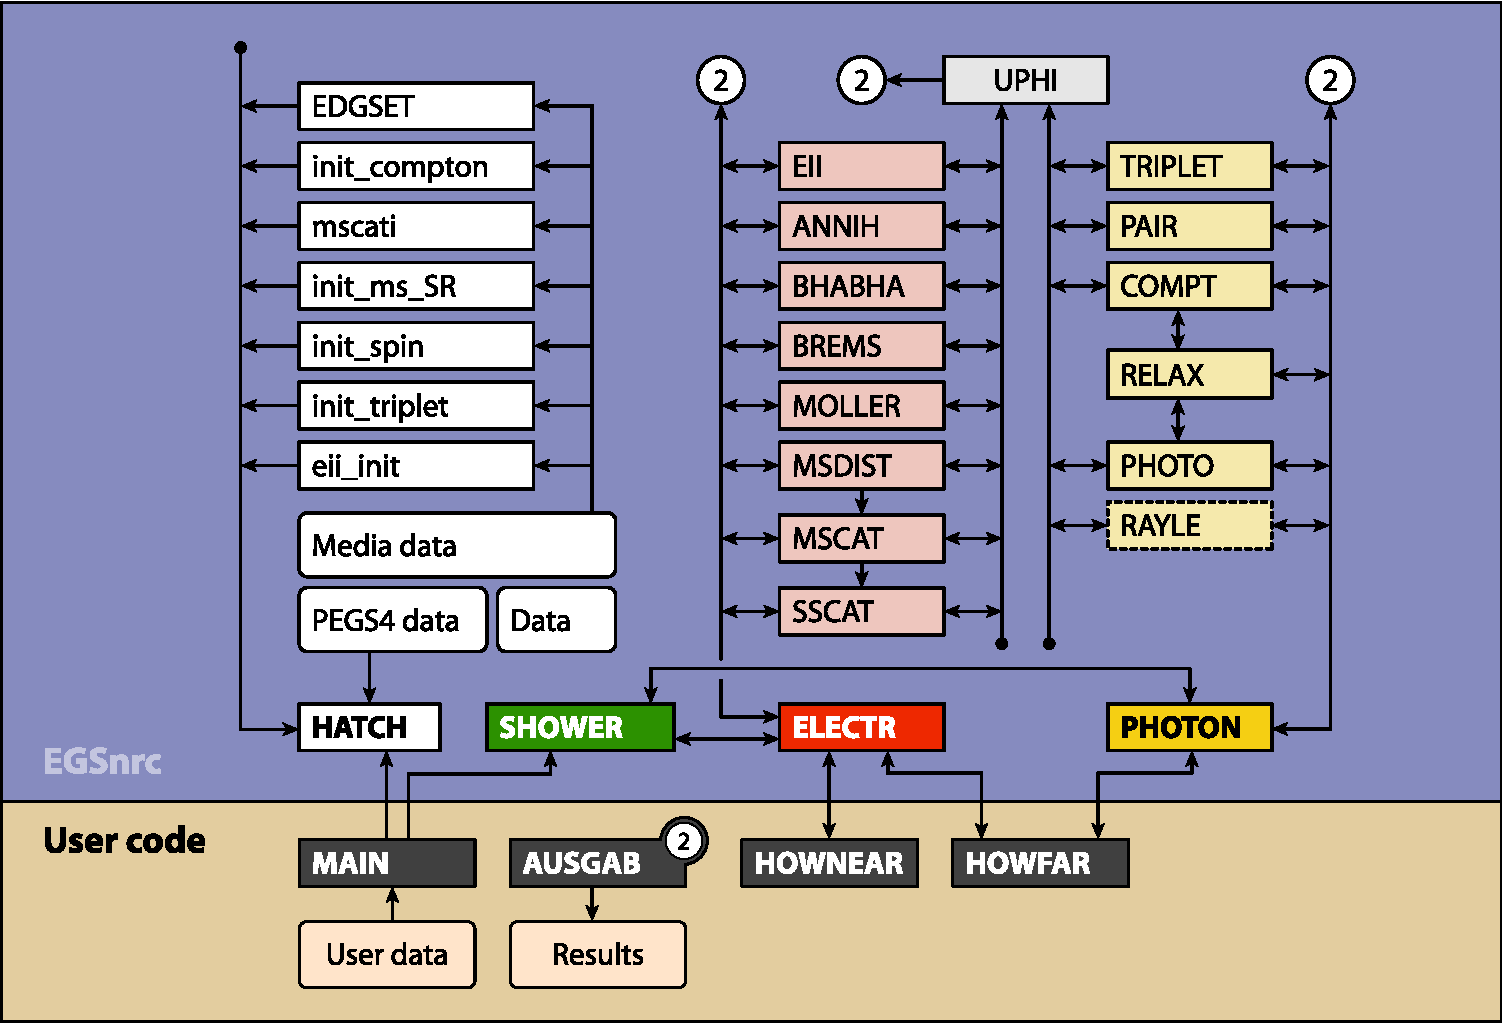
\includegraphics[width=16cm]{figures/egs-diagram}
   \end{center}
   \caption{The structure of the EGSnrc code system when used with a
user-code.}
   \label{fig_egsnrc_structure}
\end{figure}

To use EGS the user must write a ``User Code."  This consists of a
MAIN program and the subroutines {\tt HOWFAR}, {\tt HOWNEAR} and {\tt
AUSGAB}, the latter three determining the geometry and output (scoring),
respectively.  Additional auxiliary subprograms might be included in the
User Code to facilitate matters.  The user can communicate with EGS by
means of various {\tt COMMON} variables.  Usually MAIN will perform
any initialisation needed for the geometry routines, {\tt HOWFAR}
and {\tt HOWNEAR}, and sets the values of certain EGS {\tt COMMON}
variables which specify such things as names of the media to be used,
the desired cutoff energies, and the distance unit to be used (e.g.,
inches, centimeters, radiation lengths, etc.).  MAIN then calls the
{\tt HATCH} subroutine which ``hatches EGS" by doing necessary once-only
initialisation and by reading material data for the media from a data set
that had been previously created by PEGS.  This initialisation completed,
MAIN may then call {\tt SHOWER} when desired.  Each call to {\tt SHOWER}
results in the generation of one history (often referred to as a ``case").
The arguments to {\tt SHOWER} specify the parameters of the incident
particle initiating the cascade.

In addition, macro definitions can be included in MAIN in order to control
or over-ride various functions in EGS as well as in the User-Written
codes.

\index{defaults}
In EGSnrc there are many new options compared to EGS4.  The system
defaults to a set of options which will do the most complete and accurate
simulation that EGSnrc is capable of. In some cases this will imply
overkill and a reduction in efficiency with no gain in accuracy (e.g.
including atomic relaxation or bound Compton scattering for high energy
photon calculations). The user has the ability to switch things on or off
by setting various  flags.  So, eg, one could decide to run a calculation
which is nearly equivalent to using the EGS4/PRESTA electron transport
algorithm (see section~\ref{mimic}). Similarly one can choose to model
Klein Nishina Compton scattering instead of bound compton scattering by
setting a flag.

One other class of new features in EGSnrc is the implementation within the
code itself of several variance reduction techniques (range rejection and
bremsstrahlung splitting being the main two) since by doing so, a much more
efficient implementation is allowed. The user can, of course, completely
ignore these features if so desired.


      In summary, the user communicates with EGS by means of:
\begin{description}
\item[Subroutines]\mbox{}
\begin{itemize} 
\item HATCH  --- to establish media data
 
\item SHOWER --- to initiate the cascade
 
\item HOWFAR\& HOWNEAR --- to specify the geometry
 
\item AUSGAB --- to score and output the results and to control variance
reduction
 
\end{itemize} 

\item[COMMON blocks]  by changing values of variables
 
\item[Macro definitions] --- re-definition of pre-defined features.
\end{description}
 
To reiterate, we shall refer to the MAIN/HOWFAR/AUSGAB combination
(plus auxiliary subprograms and macros) as the User Code.  The following
sections discuss these things in greater detail.

\clearpage

%\newpage
\subsection{ The COMMON Blocks}

\label{common_blocks} \index{COMMON BLOCKS}
Listed here are the {\tt COMMON} blocks relevant to the user (and
relevant variables contained in them) with a brief description of their
functions.  Their usage will be discussed in more detail in subsequent
sections.  The easiest way to declare any of the {\tt COMMON} blocks is with
the {\tt COMIN} macro.  For example, {\tt COMIN/STACK,BOUNDS/;} will automatically
expand to the correct {\tt COMMON/STACK/;} and {\tt COMMON/BOUNDS/;} forms.

Note that EGSnrc is, by default, coded completely using IMPLICIT NONE. This
means that all parameters in {\tt COMMON} are all explicitly typed. See
section~\ref{implicit_none}  for more info.

\begin{table}[htb]
   \index{BOUNDS} \index{COMMON!BOUNDS} \index{ECUT}
   \index{PCUT} \index{VACDST} \index{EGS-VARIANCE-REDUCTION}
   \index{COMMON!EGS-VARIANCE-REDUCTION} \index{e\_max\_rr} \index{i\_do\_rr}
   \index{i\_play\_RR} \index{i\_survived\_RR} \index{prob\_RR}
   \index{n\_RR\_warning} \index{nbr\_split} \index{bremsstrahlung!splitting}
   \index{Russian Roulette} \index{range rejection}
   \index{bound Compton scattering}

\typeout{starting common BOUNDS table }


\begin{center}
\caption{Table describing the EGSnrc {\tt COMMON}s which are accessible to the
User.    
\label{tab_commons}
}
\begin{tabular}{ l l   p{105mm}l  |}
\hline
Common & Variable & Description \\
Block &&\\
\hline
&&\\
{\bfseries BOUNDS} & ECUT &Array of regions' charged particle
                            cutoff energies(total) in MeV.\\
       & PCUT &Array of regions' photon cutoff
                            energies in MeV.\\
       & VACDST  &   Distance to transport in vacuum (default=1.E8).\\
&&\\
\hline
&&\\
\multicolumn{3}{l}{{\bfseries EGS-VARIANCE-REDUCTION}}\\
	&e\_max\_rr &real array (\$MXREG) of maximum total energies at which 
                     to do range rejection if i\_do\_rr is set\\
	&i\_do\_rr &integer array (\$MXREG) of flags for range rejection 
                    in each region. ~~~~0$\Rightarrow$ not done (default);
                      ~~~~1$\Rightarrow$ is done.\\
&&\\
	& i\_play\_RR & flag specifying if Russian Roulette played on a
                        global basis\\
        & i\_survived\_RR & an integer flag set every time Russian Roulette
is played. If all the particles survive, it is set to 0 (which is the default
if not played at all). It is set to n if n particles were eliminated via
Russian Roulette on this interaction. It is 0 if a bound compton event is
rejected.\\
&&\\
	& prob\_RR & probability of survival if playing Russian Roulette\\
	& n\_RR\_warning & an internal counter to mark how often Russian
	Roulette is asked for with prob\_RR $\le$ 0.0. A warning is printed
       for the first \$MAX-RR-WARNING times (default 50).\\
&&\\
	&nbr\_split& For nbr\_split $>$1, nbr\_split brems photons are
sampled {every time} there is a brem interaction. The weight is reduced by
1/nbr\_split. Default value is 1.0.  If set to zero, no brem is generated
and the electron loses no energy.\\
%&&\\
\hline
    \end{tabular}
    \end{center}
    \mbox{}\hfill (cont ...)\\
    \end{table}
    \clearpage

\begin{table}[htb]
   \index{EPCONT} \index{COMMON!EPCONT} \index{EDEP} \index{TSTEP}
   \index{TUSTEP} \index{USTEP} \index{VSTEP} \index{IDISC} \index{IROLD}
   \index{IRNEW} \index{EOLD} \index{RHOF} \index{ENEW} \index{BETA2}
   \index{IAUSFL} \index{EKE} \index{ELKE} \index{GLE} \index{E\_RANGE}

\typeout{starting next common EPCONT table }
    \begin{center}
    EGSnrc COMMONs which are accessible to the User -continued\vspace*{3mm}
    \begin{tabular}{ l  l   p{105mm}l  |}
    \hline
    Common & Variable & Description \\
    Block &&\\
    \hline
&&\\
{\bfseries EPCONT}  & EDEP & Energy deposited in MeV (Double
                            Precision).\\
        & TSTEP  & Distance to next interaction (cm)\\
        & TUSTEP  & Total (curved) step length requested before check with
		geometry.\\
	& USTEP	& straight step length calculated from TUSTEP.\\
        & TVSTEP & Actual total (curved) step length to be transported.\\
	& VSTEP	& actual straight step length after truncation by geometry.\\
        & IDISC  & User discard request flag (to be set in {\tt HOWFAR}).  
                   IDISC $>$ 0 means user requests immediate discard, 
                   IDISC $<$ 0 means user requests discard after completion 
                   of transport, and IDISC=0 (default) means no user 
                   discard requested. IDISC=99 or $-$99 means generate
		   annihilation photons when positron is discarded.\\
         &IROLD  &Index of previous region.\\
         & IRNEW  & Index of new region.\\
         & RHOF   & Value of density correction (default=1) (i.e. ratio
                    of real density to that of dataset.\\
         & EOLD   &  Charged particle (total) energy
                            at beginning of step in MeV.\\
           & ENEW   & Charged particle (total) energy
                            at end of step in MeV.\\
           %& BETA2 & Beta squared for present particle.
                  %          (Note: BETA is not included).\\

           & IAUSFL & Array(29) of flags for turning on
                   various calls to {\tt AUSGAB}. See table~\ref{tab_iausflg_other}\\
           & EKE   & Electron kinetic energy in MeV.\\
           & ELKE  & Natural logarithm of EKE (this is not available for
                     a step in vacuum).\\
           & GLE   & Natural logarithm of photon energy.\\
           & E\_RANGE & For electron {\tt IARG}=0  steps, this is the range of the 
electron in the current units (see section~\ref{range_rejection}).\\
           & x[y][z]\_final & position at end of step \\
           & u[v][w]\_final & direction at end of step (only used for electrons)\\
&&\\
\hline
    \end{tabular}
    Note: the variable BETA2 is no longer available.\\
    \end{center}
    \mbox{}\hfill (cont ...)\\
    \end{table}

\clearpage

  \begin{table}[htb] 
   \index{ET-Control} \index{COMMON!ET-Control} \index{SMAXIR}
   \index{ESTEPE} \index{XIMAX} \index{SKINDEPTH\_FOR\_BCA}
   \index{TRANSPORT\_ALGORITHM} \index{SPIN\_EFFECTS} \index{EGS4}
   \typeout{starting next common ET-Control table }
   \index{BCA\_ALGORITHM}
    \begin{center}
    EGSnrc COMMONs which are accessible to the User -contnued\vspace*{3mm}
    \begin{tabular}{ l  l   p{105mm}l  |}
    \hline
    Common & Variable & Description \\
    Block &&\\
    \hline
    &&\\
    \multicolumn{2}{l}{{\bfseries ET-Control}}  &  Electron Transport Control.\\
    &&\\
	&SMAXIR	&array(\$MXREG) defining upper limit on step size in each
		region (in whatever units defined by DUNIT).(default=1.E10).\\
    &&\\
	&ESTEPE	&global energy loss constraint.(default=0.25).\\
    &&\\
	&XIMAX	&max. first GS moment per step (roughly half the average 
                MS angle squared.(default 0.5).\\
    &&\\
	&SKINDEPTH      & distance from a boundary (in elastic MFP) at which to\\
	&  ~~~\_FOR\_BCA& switch to one of the boundary crossing
		  algorithms(BCAs).(default 3).  If set 0 by the user
                  initially and BCA\_ALGORITHM = 1, then the code assigns 
                  a value consistent with 
                  BLCMIN in PRESTA-I, otherwise it is 3.0.\\
    &&\\
	&TRANSPORT& integer flag telling which transport algorithm to use.\\
 	& \_ALGORITHM	& 0$\Rightarrow$ PRESTA-II; 1$\Rightarrow$ 
                    PRESTA-I.(default 0).\\ 
    &&\\
	&BCA	&integer flag telling which BCA to use. \\
	&\_ALGORITHM  & 0$\Rightarrow$ use exact(single scattering) algorithm
                         within SKINDEPTH\_FOR\_BCA of a boundary\\
        
        &            &  1$\Rightarrow$ use multiple scattering but with
                  no lateral deflections within SKINDEPTH\_FOR\_BCA of a
                  boundary.  Default is  0.\\
    &&\\
      	&SPIN &logical variable, {\tt .true.}$\Rightarrow$ use single \&
                multiple scattering\\
	&\_EFFECTS	& theories which include relativistic spin 
               effects; {\tt .false.}
		$\Rightarrow$ use single and multiple scattering theories
                based on Rutherford scattering. (default {\tt .true.})\\ 
%to be closer to EGS4).\\
	&&\\
   \hline
   \end{tabular}
   \end{center}
\end{table}

\clearpage

\begin{table}[htb]
    \index{MEDIA} \index{COMMON!MEDIA} \index{NMED} \index{IRAYLM} \index{RLC}
    \index{RLDU} \index{RHO}
    \index{MISC} \index{COMMON!MISC} \index{MED} \index{DUNIT} \index{KMPI}
    \index{KMPO} \index{RHOR} \index{NOSCAT} \index{IRAYLR}
    \index{RANDOM} \index{COMMON!RANDOM} \index{IXX} \index{JXX} 
    \index{random number generators!seeds} \index{RANMAR} \index{RANLUX}

\typeout{****start Common MEDIA}
    \begin{center}
    EGSnrc COMMONs which are accessible to the User (cont)\vspace*{2mm}
    \begin{tabular}{ l  l   p{105mm}l  |}
    \hline
    Common & Variable & Description \\
    Block &&\\
    \hline
&&\\
{\bfseries MEDIA}	& MEDIA	&array(24,\$MXMED)  of media names.\\
	& NMED	& Number of media being used
                            (default=1).\\
          & IRAYLM & Array(\$MXMED) of flags for turning on (=1)
                            coherent (Rayleigh) scattering in
                            various media.  Set in {\tt HATCH} based
                            on values of IRAYLR.  \\
          & RLC   & Array(\$MXMED) containing radiation
                            lengths of the media in cm.  \\
	& RLDU  &  Array(\$MXMED) containing radiation
                            lengths of the media in distance
                            units established by DUNIT.\\
	&RHO	& Array(\$MXMED) containing density of the
                            media in g/cm**3.\\
        &MGE    & Array(\$MXMED) number of photon mapped energy intervals for
                  a given medium.\\
        &MEKE   & Array(\$MXMED) nuber of electron mapped energy intervals for
                  a given medium.\\
       &comp\_xsections & character*16 variable holding the name of the file\\
       && containing user-supplied Compton cross section data.\\
       &&  Full name of the file is\\
       && {\tt \$HEN\_HOUSE/data/comp\_xsections\_compton.data}.\\
       && Only used if {\tt IBCMP}=2 (bound Compton, no doppler effect).\\ 
&&\\
\hline
&&\\
{\bfseries MISC$^*$}	& MED	&Array(\$MXREG) containing medium index for
                            each region.\\
	& DUNIT	&The distance unit to be used.
                            DUNIT=1 (default) establishes all
                            distances in cm; whereas,
                            DUNIT=2.54 establishes all
                            distances in inches.\\
	&KMPI	&Fortran unit number (default=12)
                            from which to read material data.\\
	&KMPO	&Fortran unit number (default=8) on
                            which to ``echo" material data (e.g.,
                            printed output, ``dummy" output, etc.).\\
	&RHOR	&Array(\$MXREG) containing the density for each region (g/cm**3).  
		If this is different than the default density for the medium 
		for that region, the cross sections and stopping powers (with 
		the exception of the density effect) are scaled appropriately.\\
	%&NOSCAT&Number of times multiple scattering has been bypassed in 
        %       subroutine MSCAT (initialized to 0 in BLOCK DATA). This
	%       applies only if PRESTA-I or EGS4 options being used since
        %       it is never turned off in default EGSnrc.\\
	&IRAYLR	&Array(\$MXREG) of flags for turning on (=1)
                            coherent (Rayleigh) scattering in
                            various regions (default=0$\Rightarrow$ off).\\
&&\\
\hline
\multicolumn{3}{c}{$^*$ NOSCAT is no longer available since there is 
scattering on all steps.}\\
&&\\
%this common block is now found in ranmar.macros and ranlux.macros and,
%moreover, does not include ixx, jxx
%{\bfseries RANDOM}
%	&IXX,JXX & When using the RANLUX random number generator, the user
%does not pass anything via this {\tt COMIN}. When using RANMAR, IXX and JXX
%are passed. Initially random number seeds, these 
%become pointers once the generator is initialized. 0$<$IXX$<=$31328 and 0$<$JXX$<=$30081.\\
\hline
    \end{tabular}
    \end{center}
    \mbox{}\hfill (cont ...)\\
    \end{table}
    \clearpage



\begin{table}[htb]

   \index{STACK} \index{COMMON!STACK} \index{E} \index{X,Y,Z} \index{U,V,W}
   \index{DNEAR} \index{WT} \index{IQ} \index{IR} \index{NP} \index{NPold}
   \index{LATCH} \index{LATCHI}


   \index{THRESH} \index{COMMON!THRESH} \index{RMT2} \index{RMSQ} \index{AP}
   \index{UP} \index{AE} \index{UE} \index{TE} \index{THMOLL} \index{\$MXMED}
   \index{\$MXSTACK} \index{variance reduction}

\typeout{****start COMMON STACK}

    \begin{center}
    EGSnrc COMMONs which are accessible to the User (cont).
    \begin{tabular}{ l  l   p{105mm}l  |}
    \hline
    Common & Variable & Description \\
    Block &&\\
    \hline
&&\\
{\bfseries STACK}	&	&Note: This COMMON block contains the
                            information about the particles
                            currently in the shower.  All
                            of the following variables are
                            arrays(\$MXSTACK) except {\tt NP, NPold}  and
                            {\tt LATCHI}.\\
	&E	&Total energy in MeV (Double
                            Precision).\\
	& X,Y,Z & Position of particle in units
                            established by DUNIT.\\
	&U,V,W	&Direction cosines of particle (not
                            necessarily normalized if table lookups used
                      for sines---see section~\ref{step_1}).\\
	&DNEAR	&A lower bound of distance from
                            (X,Y,Z) to nearest surface of
                            current region.\\
	& WT	&Statistical weight of current particle(default=1.0).  To be 
		used in conjunction with variance reduction techniques as 
                determined by user.\\
	& IQ	&Integer charge of particle
                            (+1,0,-1).\\
	&IR	&Index of particle's current region.\\

	& NP	& The stack pointer (i.e., the particle currently being pointed
                            to).  Also, the number of particles on the stack.\\

	&NPold	& Value of {\tt NP} prior to an interaction (to test how many
		particles created see section~\ref{stack_status}).\\

	&LATCH	&An integer variable for use to track histories.\\

	&LATCHI	&Initial value of LATCH(1) when shower called.\\
&&\\
\hline
&&\\
{\bfseries THRESH}	&RMT2	&Twice the electron rest mass
                            energy in MeV.\\
	&RMSQ	& Electron rest mass energy squared
                            in MeV-squared.\\
	&AP	&Array(\$MXMED) containing PEGS lower photon
                            cutoff energy for each medium in
                            MeV.\\
	&UP	& Array(\$MXMED) containing PEGS upper photon
                            cutoff energy for each medium in
                            MeV.\\
	&AE	&Array(\$MXMED) containing PEGS lower charged
                            particle cutoff energy for each
                            medium in MeV.\\
	&UE	&Array(\$MXMED) containing PEGS lower charged
                            particle cutoff energy for each
                            medium in MeV.\\
	&TE	&Same as AE except kinetic energy
                            rather than total energy.\\
	&THMOLL	&Array(\$MXMED) containing the Moller thresh-
                            hold energy (THMOLL=AE+TE) for
                            each medium in MeV.\\
&&\\
\hline
    \end{tabular}
    \end{center}
    \mbox{}\hfill (cont ...)\\
    \end{table}
    \clearpage

\begin{table}[htb]
   \index{UPHIOT} \index{COMMON!UPHIOT} \index{THETA} \index{SINTHE}
   \index{COSTHE} \index{SINPHI} \index{COSPHI} \index{PI} \index{TWOPI}
   
   \index{USEFUL} \index{COMMON!USEFUL} \index{MEDIUM} \index{MEDOLD}
   \index{RM} \index{PRM} \index{PRMT2} \index{PZERO}
   \index{USER} \index{COMMON!USER}

    \begin{center}
    EGSnrc COMMONs which are accessible to the User (cont).
    \begin{tabular}{ l  l   p{105mm}l  |}
    \hline
    Common & Variable & Description \\
    Block &&\\
    \hline
    &&\\
    {\bfseries UPHIOT}	&THETA	&Collision scattering angle (polar).\\
	&SINTHE	& Sine of THETA.\\
	&COSTHE & Cosine of THETA.\\
	&SINPHI	&Sine of PHI (the azimuthal
                            scattering angle of the collision).\\
	&COSPHI	& Cosine of PHI.\\
	&PI	& Pi.\\
	&TWOPI	& two Pi.\\
        &PI5D2  & 2.5 $\times$ Pi.\\
    &&\\
    \hline
    &&\\
    {\bfseries USEFUL}	&MEDIUM	&Index of current medium.  If
                            vacuum, then MEDIUM=0.\\
	&MEDOLD	&Index of previous medium.\\
	&RM	&Electron rest mass energy in MeV.(see also THRESH)\\
	&PRM	& ``Precision" electron rest mass
                            energy in MeV (Double Precision).\\
	&PRMT2	&Twice PRM (Double Precision).\\
	&PZERO	&precise 0.0 (Double Precision).\\
    &&\\
   \hline
    &&\\
    {\bfseries USER} & & Null by default but available in ELECTR, PHOTON
                     and HATCH to allow users to pass data into the
        transport routines (eg geometry data, variance reduction data
etc).\\
    &&\\
   \hline
&&\\
{\bfseries CH-Steps} & {\tt count\_pII\_steps} & keeps a count of number of
electron steps taken using the PRESTA-II multiple scattering model
(real*8).\\
& {\tt count\_all\_steps} & counts all electron steps (real*8).\\
& {\tt is\_ch\_step} & a logical variable set to true if the current electron\\
&& step is a condensed history ({\em i.e.} using PRESTA-I or PRESTA-II multiple\\
&& scattering theory) step.\\
&&\\
   \end{tabular}
   \end{center}
\end{table}

\clearpage

As well as the {\tt COMIN}s described above, there are several {\tt COMIN}s which are
normally just internal to EGSnrc, which have one or two variables which the
user may require access to in order to control various options within
 EGSnrc.  In an ideal world these would all be gathered into a single
{\tt COMIN}
but that would make compatibility with EGS4 user codes even more difficult
to achieve.  We have adopted this compromise solution which changes as
little as possible of what has grown up historically with EGS4.  So, for
example the parameters {\tt IEDGFL}, {\tt IPHTER}, 
{\tt IBRDST} and {\tt IPRDST} have not been
moved and the new parameters introduced with EGSnrc have similarly been
placed in those {\tt COMIN}s associated with the physics being controlled.
Table~\ref{tab_new_commons} summarizes these {\tt COMIN}s which are needed to
control further the transport parameters.  Note that the user code can
ignore these {\tt COMIN}s completely if you are satisfied with the default
settings for photon and electron transport in EGSnrc.
\index{EGS4}
\index{IPRDST} \index{IBRDST}
\clearpage

\clearpage
 \begin{table}[hb]
\index{COMINs}
\index{ibr\_nist}
\index{EDGE}
\index{COMMON!EDGE}
\index{IEDGFL}
\index{IPHTER}
\index{photoelectric interactions}
\index{fluorescence}
\index{photoelectric interactions!angular distribution}
\index{COMMON!COMPTON-DATA}
\index{COMPTON-DATA}
\index{Compton effect}
\index{bound Compton scattering}
\index{Doppler effects}
\index{IBCMP}
\index{BREMPR}
\index{COMMON!BREMPR}
\index{IBRDST}
\index{IPRDST} \index{EGS4}
\index{bremsstrahlung!production}
\index{bremsstrahlung!angle}
\index{pair production}
\index{Coster-Kronig electrons}
\index{Koch and Motz}
\index{RAYLEIGH\_INPUTS}
 \begin{center}
 \label{tab_new_commons}
 \caption{EGSnrc {\tt COMMON}s which are optionally accessible to the user. Not all
elements in each {\tt COMIN} are described since many of them are not
to be accessed by the user.\vspace*{5mm} }
 \begin{tabular}{ l  l   p{105mm}l  |}
 \hline
 Common & Variable & Description \\
  Block &&\\
    \hline
&&\\
{\bfseries EDGE}	&IEDGFL	& integer array (\$MXREG) specifying whether
relaxation of the atom is modelled after photo-effect or bound compton
events (at present). When on, fluorescent photons, Auger electrons and
Coster-Kronig electrons above threshold are modelled explicitly. When not
on, the photoelectron acquires the entire energy of the incident photon
(contrary to what happened in EGS4).  (1$\Rightarrow$ yes (default),
0$\Rightarrow$ no).\\
	&IPHTER	& integer  array (\$MXREG) specifying whether to sample the
         angular distribution of photo-electrons in each region
(1$\Rightarrow$ yes (default),
0$\Rightarrow$ no) .\\
&&\\
% do we want to list more from this common block here 
\hline
&&\\
{\bfseries COMPTON-} &IBCMP &integer array (\$MXREG) specifying whether to 
                    include \\
{\bfseries ~~~~~~DATA} & & binding and Doppler broadening effects in Compton 
            scattering events (1$\Rightarrow$ yes (default), 0$\Rightarrow$ no).\\
                  & radc\_flag & integer flag for radiative Compton corrections.\\
                 && 0$\Rightarrow$ off (default), 1$\Rightarrow$ on.\\
&&\\
\hline
&&\\
{\bfseries BREMPR} &  IBRDST & flag determining how angle of a brem
photon is selected.  0$\Rightarrow$ sample leading term of the angular
dist'n; 1$\Rightarrow$ sample the ang. distn. of Koch and Motz. Default=1.
For $<$0, the angle is the same as that of the photon so user can use a
call to {\tt AUSGAB} to set the angle.\\

& IPRDST &flag determining how the electron/positron angles are selected
after pair production. 0$\Rightarrow$ use the fixed angle approximation of
EGS4. 1$\Rightarrow$ sample the leading term in the angular distribution 
(fast and good enough). 2$\Rightarrow$ sample the complete angular distribution.  Default is 1.\\

& ibr\_nist& integer flag determining which differential photon cross section 
to sample when brem occurs.\\
&& 0$\Rightarrow$ use Bethe-Heitler as done in EGS4. This is the default.\\
&& 1$\Rightarrow$ use NIST data base from ICRU Report 37.\\
& itriplet & set to 1 to explicitly simulate triplet events (default is 0).\\
& pair\_nrc & flag determining which pair production cross-sections are used.\\
&& 0$\Rightarrow$ use Bethe-Heitler cross-sections (default).\\
&& 1$\Rightarrow$ use NRC cross-sections \\
&&\\
\hline
    \end{tabular}
    \end{center}
    \mbox{}\hfill (cont ...)\\
    \end{table}
    \clearpage

\begin{table}[htb]

   \index{EII-DATA} \index{RAYLEIGH\_INPUTS} \index{EGS-IO}
   \index{electron impact ionization!inputs}
   \index{Rayleigh custom form factors}
    \index{I/O file units}
    \begin{center}
    EGSnrc internal COMMONs optionally accessible to the User (cont).
    \begin{tabular}{ l  l   p{105mm}l  |}
    \hline
    Common & Variable & Description \\
    Block &&\\
    \hline
&&\\
{\bfseries EII-DATA} & {\tt eii\_flag} & flag determining which, if any, electron
impact ionization theory is used.\\
&& 0$\Rightarrow$ turn electron impact ionization off (the default).\\
&& 1$\Rightarrow$ use Kawrakow's EII theory\cite{Ka02b}.\\
&& 2$\Rightarrow$ use the theory of Casnati\cite{Ca82}.\\
&& 3$\Rightarrow$ use the theory of Kolbenstvedt\cite{Gr65a}.\\
&& 4$\Rightarrow$ use the theory of Gryzinski\cite{Ko67}.\\
&&\\
\hline
&&\\
{\bfseries RAYLEIGH} & {\tt iray\_ff\_media} & array (with dimension
{\tt \$MXMED}) containing the names of the\\
{\bfseries \mbox{~~~~}\_INPUTS}&& media (must appear in the PEGS4 data) for which custom Rayleigh
form factors are to be provided.  Otherwise, the medium
uses the default atomic form factor.\\
& {\tt iray\_ff\_file} & array (with dimension {\tt \$MXMED}) containing
full names ({\em} including directory path) of files specifying
custom form factors.  {\tt iray\_ff\_file(i)} corresponds to
{\tt iray\_ff\_media(i)}.\\
&&\\
\hline
&&\\
{\bfseries EGS-IO} & {\tt file\_extensions} & character array (with
dimension {\tt \$mx\_units}; default=20) containing
extensions of files specified in the code's {\tt .io} file.
Maximum extension length is {\tt \$max\_extension\_length} (default=10 characters).\\
& {\tt file\_units} & integer array (with
dimension {\tt \$mx\_units}) where {\tt file\_units(i)} specifies Fortran unit number associated with
the file having extension {\tt file\_extensions(i)}.\\
& {\tt user\_code} & the name of the user code (max. length = 64 chars).\\
& {\tt input\_file} & the name of the input file.  Includes directory path but
no extension (max. length=256 chars).\\
& {\tt output\_file} & same as above but for the output file.\\
& {\tt pegs\_file} & the name of the pegs data file.  Includes directory path
and extension (max. length=256 chars).\\
& {\tt hen\_house} & the user's {\tt \$HEN\_HOUSE} directory (max. length=128 chars).\\
\hline
    \end{tabular}
    \end{center}
    \mbox{}\hfill (cont ...)\\
    \end{table}
    \clearpage

\begin{table}[htb]

   \index{EGS-IO}
   \index{I/O file units}

    \begin{center}
    EGSnrc internal COMMONs optionally accessible to the User (cont).
    \begin{tabular}{ l  l   p{105mm}l  |}
    \hline
    Common & Variable & Description \\
    Block &&\\
    \hline
\hline
{\bfseries EGS-IO} & {\tt egs\_home} & the user's {\tt \$EGS\_HOME} directory (max. length=128 chars).\\
\mbox{~~~}{\bfseries (cont)}& {\tt work\_dir} & the temporary working directory created in the user's
{\tt \$EGS\_HOME/user\_code} during a run (max. length=128 chars).\\
& {\tt host\_name} & the name of the machine being run on (max. length=64 chars).\\
& {\tt n\_parallel} & if $>$0, the total number of parallel jobs.\\
& {\tt i\_parallel} & if $>$0, the number of the current parallel job.\\
& {\tt first\_parallel} & the first parallel job number (default=1).\\
& {\tt n\_max\_parallel} & max. number of parallel jobs executing simultaneously
(updated during run).\\
& {\tt n\_chunk} & no. of histories per calculation chunk during a parallel run.
(currently not used).\\
& {\tt n\_files} & no. of files specified in the {\tt user\_code.io} file
(max={\tt \$mx\_units}).\\
& {\tt i\_input} & unit no. for standard input, or the {\tt .egsinp} file (default=5).
Note this is used in BEAMnrc to prevent unit collisions when used as
a shared library source.\\
& {\tt i\_log} & unit no. for standard output, or the {\tt .egslog} file (default=6).
Used in BEAMnrc to prevent unit collisions when used as a
shared library source.\\
& {\tt i\_incoh} & unit numbers for data files containing Compton (default=78),\\
& {\tt i\_nist\_data} & bremsstrahlung (default=76), multiple scattering (default=11),\\
& {\tt i\_mscat} & photon cross-section (default=79), and photon relaxation\\
& {\tt i\_photo\_cs} & data (default=77), respectively.  Variable unit numbers\\
& {\tt i\_photo\_relax} & are used to allow BEAMnrc shared library sources to
access these files as well.\\
& {\tt xsec\_out} & =0 $\rightarrow$ do not output file {\tt user\_code.xsections} containing photon cross-section data (default).\\
&& =1 $\rightarrow$ output file containing photon cross-section data.\\
& {\tt is\_batch} & logical variable set to {\tt .true.} if this is a batch
job.\\ 
&&\\
\hline
&&\\ 
\end{tabular}
\end{center}
\end{table}
\clearpage

\subsection{The Sequence of Operations}
\index{sequence of operations}
\index{steps}
\index{steps!order}
 
The sequence of operations needed for the correct operation of EGS is
shown below.

\begin{description}
\item[Step 0.]  {\tt call egs\_init} for file initialization (see
PIRS-877 for details\cite{Ka03}). 
\item[Step 1.]  User Over Ride Of EGS Macros and Defaults (\ref{step_1})
\item[Step 2.]  Pre-{\tt HATCH} Call Initialisation (\ref{step_2})
\item[Step 3.]  {\tt HATCH} Call (\ref{step_3})
\item[Step 4.]  Initialisation For {\tt HOWFAR} \& {\tt HOWNEAR} (\ref{step_4})
\item[Step 5.]  Initialisation For {\tt AUSGAB} (\ref{step_5})
\item[Step 5b.] Initialisation For Variance Reduction (\ref{step_5b})
\item[Step 6.]  Determination Of Incident Particle Parameters
              (\ref{step_6})
\item[Step 7.]  SHOWER Call (\ref{step_7})
\item[Step 8.]  Output Of Results (\ref{step_8})
\item[Step 9.] {\tt call egs\_finish} as the last executable statement. See 
ref~\cite{Ka03} for details. Properly closes files and places them back on
the user-code's directory.
\end{description}
\vspace*{-4mm}
 The following are restrictions on the order of these
 operations:
\vspace*{-4mm}
\begin{enumerate}
\item  Step 1 must precede use of any EGS macros by the user.
\item Step 0 should be the first executable statement and thus is usually
after Step 1 and possibly in Step 2.
\item  Step 2 must precede Step 3.
\item Steps 3 through 6 must precede Step 7.
\item Step 7 may be repeated as often as desired, depending on whether 
  information on single showers or many showers is desired (e.g., for shower 
  fluctuation or conversion efficiency calculations).
\item At least one Step 7 must precede the first Step 8.
\end{enumerate}
 
Details for the above steps are given in the following sub-sections.

It is strongly advised that the user echo {\bfseries ALL} input parameters
into the output listing file to ensure that the listing has a complete
record of the run.  From extensive experience we have found that this is
essential and very valuable.
 
 
 \subsubsection{User Over Ride Of EGS Macros and Defaults (Step 1)}
\label{step_1}
\index{Step 1: Override macros}
 
EGS macros which the user might want to over-ride include the following:
 
\paragraph{{\tt \$CALL-HOWNEAR(\#)}}
\label{hownear_macro}
\index{EGS4}
\mbox{}\\
For compatibility with  EGS4/PRESTA user-codes, the use of {\tt SUBROUTINE
HOWNEAR} has been left as a macro call in EGSnrc.  
There is no default definition of the macro but the following is suggested:
\begin{verbatim}
REPLACE {$CALL-HOWNEAR(#);} WITH {CALL HOWNEAR({P1},X(NP),Y(NP),Z(NP),IRL);}
\end{verbatim}
The user may choose to define an equivalent macro.
The parameter that must be returned by the macro 
is the shortest distance to any
boundary from the current position. See
section~\ref{hownear}(page~\pageref{hownear}) which
specifies the macro or subroutine completely.  There is also some
discussion in section~\ref{hownear_change} (page~\pageref{hownear_change}).
\index{HOWNEAR}
\index{SUBROUTINE HOWNEAR}
\index{\$CALL-HOWNEAR}

\paragraph{{\tt \$IMPLICIT-NONE, \$REAL, \$INTEGER}}
\label{implicit_none}
\mbox{}\\
The EGSnrc system is now coded with {\tt \$IMPLICIT-NONE;} (which defaults
to {\tt IMPLICIT NONE;}) in all
subroutines. This means that any time the user is passing a variable
into the EGSnrc system by means of adding to a {\tt COMIN} definition, one
must explicitly specify the type of that variable.  To turn this feature off one adds
the following statement to the user code:
\begin{verbatim}
                REPLACE {$IMPLICIT NONE;} WITH {;}
\end{verbatim}
It is strongly recommended that user codes adopt the use of {\tt
\$IMPLICIT NONE;} since it catches many coding errors and prevents
accidental collision of variables.

\index{\$IMPLICIT-NONE}
\index{\$REAL}
\index{\$INTEGER}
\index{IMPLICIT-NONE}
\index{REAL}
\index{INTEGER}

In addition to using {\tt \$IMPLICIT NONE;}, the EGSnrc system has used
the macros {\tt \$REAL} and {\tt \$INTEGER} everywhere to define real
and integer variables as well as using generic intrinsic functions such
as MAX and MIN.  By default {\tt \$REAL} and {\tt \$INTEGER} are defined
as {\tt REAL*8} and {\tt INTEGER*4}.  However, to make the entire code
run in single precision, one can add the macro:
\begin{verbatim} 
                REPLACE {$REAL} WITH {;REAL*4}
\end{verbatim}
However, this requires that all type declarations in the user code also use
the macros {\tt \$REAL} and {\tt \$INTEGER} everywhere.  With 64 bit
machines, one might as well use the {\tt REAL*8} default.

\paragraph{Array Dimensions}
\index{\$MXMED}
\index{\$MXREG}
\index{\$MXSTACK}
\begin{description} 
\item[{\tt \$MXMED}]   Maximum number of media (default=10).
\item[{\tt \$MXREG}]   Maximum number of regions (default=2000).
\item[{\tt \$MXSTACK}]  Maximum number of particles on the {\tt STACK} at once
(default = 40).
\end{description} 
For example, to extend the number of media to 25, include the following 
statement in the User Code.
\begin{verbatim}
         REPLACE {$MXMED} with {25} 
\end{verbatim}
Note that there are often array dimensions defined by the user for scoring
arrays and these should be defined at this step as well.
 
\paragraph{Random Number Initialisation}
\label{rng_init}

\index{random number generators!initialisation}
\index{\$INITIALIZE RNG USING} \index{luxury level} \index{iseed}
\index{RANMAR} \index{RANLUX}
\mbox{}\\
By default the RANLUX random number generator requires no
initialisation. However, to use a luxury level different from the default
of 1,  or a different initial seed, then you must initialize it using:
\begin{verbatim}
         $INITIALIZE RNG USING luxury_level AND iseed;
\end{verbatim}
The {\tt luxury levels} are from 0 to 4, but the value 0 is known to cause
problems with EGSnrc calculations. The value of {\tt iseed} is from 1 to
1073741824 (2$^{30}$).

If you have selected the RANMAR random number generator (via the {\tt
.configuration} file, then it MUST be initialized before it is first used.
This can be accomplished by including the statement:
\begin{verbatim}
        $RNG-INITIALIZATIION;
\end{verbatim} 
which initializes RANMAR using whatever the current values of {\tt IXX} and
{\tt JXX} are and uses default values if they have not been set (they are
passed in {\tt COMIN/RANDOM/;}. Alternatively, one can use:
\begin{verbatim}
         $INITIALIZE RNG USING IXX AND JXX;
\end{verbatim}
which accomplishes the same thing. The values are restricted to:
{\tt 0 $<$ IXX $\le$ 31328} and {\tt 0 $<$ JXX $\le$ 30081} and 0 values
are set to defaults.

The random number generator may be initialized at any step prior to the
call to {\tt SHOWER} in step 7, or prior to the first use in the user code.

For a complete discussion of these and other issues about the random number
generators, see section~\ref{rngs} below (page~\pageref{rngs}).
\index{random number generators!initialisation}

 
\paragraph{{\tt \$SET-RHOF}}

\label{set_rhof}
\index{RHOR}
\index{density changes}
\index{RHOF}
\index{\$SET-RHOF}
\mbox{}\\
Section~\ref{RHOF_RHOR}(page~\pageref{RHOF_RHOR}) explains the use of {\tt
RHOF}.  On each step, EGSnrc calls a macro {\tt  \$SET-RHOF} which
evaluates the ratio of the density at that point to the density given in
the PEGS4 data file for the material in that region. Setting {\tt RHOR}
allows you to scale the density throughout a region to some new density. If
you have a problem in which the density is varying within the region, this
can be handled by replacing the default macro:
\begin{verbatim}
         REPLACE {$SET-RHOF;} WITH {RHOF=RHOR(IRL)/RHO(MEDIUM);}
\end{verbatim}  
by whatever code you want to return the local density ratio. If, on the
other hand you do not use density scaling at all in your code, you should
replace the default with:
\begin{verbatim}
         REPLACE {$SET-RHOF;} WITH {RHOF = 1.0;}
\end{verbatim} 
since this saves a division on every step.


\paragraph{Sines and Cosines}
 
\index{sine}
\index{cosine}
\index{table lookup sines}
\mbox{}\\
To increase calculational speed, sines and cosines were not always
determined by function (e.g., {\tt SINTHE= SIN(THETA))} in the default
 EGS4.  Instead, the sine was looked-up in a sine-table and the cosine
was determined from the sine.  However, this was found to lead to very
small errors for angles very close to 0 degrees\cite{LR94a}.  This can
be overcome but with modern computers the speed of the sine and cosine
evaluations is as fast as the table lookup method so we have reverted back
to direct function evaluations.  For slightly older machines, the table
lookup feature saved as much as 40\% of the CPU time.  If you happen
to be using one of these machines, it is worthwhile to use the table
lookup method unless small angles are critical to you.  To re-implement
it, define the following two macros in STEP 1.  
\begin{verbatim}
REPLACE {$EVALUATE#USING SIN(#);} WITH {{P1}=SIN1(L{P2})*{P2}+SIN0(L{P2});}}
REPLACE {$SET INTERVAL#,SINC;} WITH {L{P1} = SINC1*{P1} +SINC0;}}} 
\end{verbatim}
%\cen{{\tt REPLACE \{\$EVALUATE\#USING SIN(\#);\} WITH \{\\
      %~~~~~~~~\{P1\} = SIN1(L\{P2\})*\{P2\} + SIN0(L\{P2\}) ;\} }\\
%{\rm and\\}
 %{\tt REPLACE \{\$SET INTERVAL\#,SINC;\} WITH \{L\{P1\} = SINC1*\{P1\}
%+SINC0;\}}} 
The reader is referred to the Mortran3 User's Guide as an
aid in understanding the macros (see section~\ref{UGM3}).

 
It should be pointed out that due to the precision involved in the table
look-up method, the direction cosines can become slightly unnormalized.
Depending on the problem at hand, this can lead to incorrect results---such
as when two direction cosines are simultaneously involved in an angular
sort of particles.  The problem can generally be remedied by renormalizing
the direction cosines prior to using them.

 
\paragraph{Charged Particle Transport}
\index{charged particle transport}
\index{electric fields}
\index{magnetic fields}
\index{\$CHARGED-TRANSPORT}
\mbox{}\\
The pattern {\tt \$CHARGED-TRANSPORT} has been included in subroutine ELECTR in
order to allow transport of the charged particles by other means than used
in this version.  For example, \cen{ {\tt REPLACE \{\$CHARGED-TRANSPORT;\}
WITH \{CALL MYTRAN;\}}} could be included in Step 1 of the User Code,
and an appropriate subroutine MYTRAN would need to be provided by
the user.  For a detailed discussion of one such implementation, see
ref\cite{Bi89a,Bi93}



\subsubsection{Pre-HATCH Call Initialisation (Step 2)}
\label{step_2}
\index{Step 2: pre-hatch}
 
This step consists of setting EGS {\tt COMMON} variables that are used by {\tt
HATCH}
in its initialisation operations.  All of these variables are initialized
to some reasonable value in the BLOCK DATA subprogram.  Therefore, if
different values are desired they should be set with executable code (as
opposed to another BLOCK DATA).  Concurrently, the various {\tt COMMON} blocks
(i.e., BOUNDS, MEDIA, MISC) will have to be included in the declaration
section of the MAIN program of the User Code.  

\index{get\_transport\_parameter}
If the user code reads an input ({\tt .egsinp}) file for defining
the simulation geometry, sources, etc, then
{\tt COMMON} variables controlling Monte Carlo transport are accessible to the user
through the subroutine {\tt get\_transport\_parameter}.  This can
be called by a user code prior to calling {\tt HATCH} provided that
the user code includes the files\\
 {\tt \$HEN\_HOUSE/src/get\_inputs.mortran}
(contains the actual {\tt get\_transport\_parameter} subroutine) and
{\tt \$HEN\_HOUSE/src/transportp.macros} (contains necessary macros)
in the {\tt SOURCES} list defined in either {\tt Makefile} or
{\tt user\_code.make}.
Note that {\tt \$HEN\_HOUSE/src/transportp.macros} must occur before
{\tt \$HEN\_HOUSE/src/get\_inputs.mortran} and
{\tt \$HEN\_HOUSE/src/egsnrc.mortran} in the list of {\tt SOURCES}.

The call to {\tt get\_transport\_parameter} is:
\begin{verbatim}
call subroutine get_transport_parameter(6)
\end{verbatim}
where the parameter ``6'' instructs the subroutine to read the
transport parameters from the {\tt .egsinp} file and to echo the parameters
to the screen (or {\tt .egslog} file if running in batch).

Within the {\tt .egsinp} file, the transport parameter settings must
appear between the delimiters:
\begin{verbatim}
:Start MC Transport Parameter:

:Stop MC Transport Parameter:
\end{verbatim}

The general format of inputs for {\tt get\_transport\_parameter} is
a text line followed by ``='' and then the value(s) that the user
wants to assign to the particular parameter.  Note that 
these inputs are case insensitive.

For some more information about {\tt get\_transport\_parameters} along
with a printout of the input description appearing at the top of
the code, see the PIRS-702 User Code Manual\cite{Ro03}.

The {\tt COMMON} block variables which must be initialized before calling
{\tt HATCH}, along with the method to set them if using the
{\tt get\_transport\_parameter} subroutine (where applicable) are: 
\begin{description}
\item[NMED]  This must be initialized to the number of media to be used in
the shower generation (default=1).

 
\item[MEDIA] This array contains the names of the media required and
is dimensioned\\{\tt MEDIA(24,\$MXMED)}, where {\tt \$MXMED} is an EGS
macro that is currently defined to be 10 (default), and whose value is
the maximum number of media for which array space has been allocated
(see section~\ref{step_1} above).  The media names are stored in MEDIA in
alphameric field specification A1 to ensure portability.  Each medium name
is 24 characters long.  For the convenience of users compiling with EGS'
macros, there is a macro to generate A1 strings.  For example, \cen{{\tt
\$S'STRING'} expands to {\tt 'S','T','R','I','N','G'.}}
\index{MEDIA} \index{\$S}

One way of implementing this in the User Code is demonstrated in the next
example, which is for three media: lead, steel, and air at NTP.  A
temporary array is declared and initialized in MAIN by:
 \cen{{\tt CHARACTER*4 TEMP(24,3)/\$S'PB',        22*' ', \$S'STEEL',
19*' ', \$S'AIR AT NTP',14*' '/;}}
and at Step 2 one puts
\cen{ {\tt NMED=3;~~~~~"number of media used"\\
           ~~~~~~~~~~~~  DO J=1,NMED [DO I=1,24 [MEDIA(I,J)=TEMP(I,J);]]}}
 
\index{MED}
\item[MED] This array, which is dimensioned {\tt MED(\$MXREG)}, contains the
medium indices for each region (default values are 1 for all {\tt \$MXREG}).  A
medium index of zero means a region is filled with a vacuum. For instance,
if we consider the three media example above along with vacuum to define
four regions, in Step 2 of the User Code we might have: 
\begin{verbatim}
             MED(1)=3;  "first region is air at NTP"
             MED(2)=1;  "second region is lead"
             MED(3)=0;  "third region is vacuum"
             MED(4)=2;  "fourth region is steel"
\end{verbatim}
 
\index{ECUT}
\index{PCUT}
\index{AE}
\index{AP}
\item[ECUT and PCUT] These arrays contain the cutoff energies (in MeV) for
charged particles and photons, respectively, for each region.  They are
dimensioned {\tt ECUT(\$MXREG)} and {\tt PCUT(\$MXREG)} and are given
temporary (default) values of 0.0 in {\tt BLOCK DATA}.  At the time that
data for each medium are generated in the preprocessing code (PEGS), two
parameters ({\tt AE} and {\tt AP}) are set to the lowest energies at which
it will be desired to transport electrons and photons.  When the EGS
subroutine {\tt HATCH} is called, these {\tt AE} and {\tt AP} values are
read in and {\tt HATCH} upgrades the values of {\tt ECUT} and {\tt PCUT}
such that the maximum of the current {\tt (ECUT,AE)} (and {\tt (PCUT,AP))}
is chosen.  Therefore, by assigning values of {\tt ECUT} and {\tt PCUT}
prior to the {\tt HATCH} call, the user can raise (but not lower) the
cutoff energies in this manner.  For instance, consider the four region
example from above.  The statement
\begin{verbatim}
             DO I=1,3 [ECUT(I)=10.0; PCUT(I)=100.0;]
\end{verbatim}
when put in Step 2 of the User Code results in charged particle histories
being terminated at 10.0 MeV (total energy) and photon histories being
terminated at 100.0 MeV in the first three regions only.  In the fourth
region the respective cutoffs are set by {\tt AE} and {\tt AP} as established by PEGS.
Of course COMMON/BOUNDS/ will have to be declared in the routine that calls
{\tt HATCH} in order to pass ECUT and PCUT to {\tt HATCH}.  Combined with
{\tt COMMON/MEDIA/}
and {\tt COMMON/MISC/}, the macro declaration might look like
\begin{verbatim}
                COMIN/BOUNDS,MEDIA,MISC/;
\end{verbatim}

If using the {\tt get\_transport\_parameter} subroutine, then global 
values of {\tt ECUT} and {\tt PCUT} can be set using:
\begin{verbatim}
Global ECUT= ECUT
Global PCUT= PCUT
\end{verbatim}

\index{DUNIT}
\item[DUNIT] This parameter determines the unit of distance to be used in
the shower simulation (the default is cm if {\tt DUNIT=1.0}).  On input to {\tt
HATCH},
this parameter will be interpreted as follows:
\begin{description} 
\item[DUNIT $>$ 0] means that {\tt DUNIT} is the length of the distance unit
expressed in centimeters.  For example, setting {\tt DUNIT}=2.54 would mean that
the distance unit would be one inch.

 \item[DUNIT $<$ 0] means that the absolute value of {\tt DUNIT} will be
interpreted as a medium index.  The distance unit used will then be the
radiation length for this medium, and on exit from {\tt HATCH}, {\tt DUNIT} will be
equal to the radiation length of that medium in centimeters.  The obvious
use of this feature is for the case of only one medium with {\tt DUNIT}=-1.  Then
the shower is expressed entirely in radiation lengths of the first medium.

 
\index{distance unit}
The distance unit used by PEGS is the radiation length.  After {\tt HATCH}
interprets {\tt DUNIT}, it scales all distance- type data from PEGS in the proper
way, so that all subsequent operations in EGS will be correctly performed
with all distances in units of {\tt DUNIT} (default value: 1.0 cm).
\end{description}

 
\index{IRAYLR}
\index{Rayleigh scattering!turning on}
\item[IRAYLR] The elements of this integer array (dimensioned {\tt
IRAYLR(\$MXREG)} and passed in\\ {\tt COMMON/MISC/)} are to be set to 1
prior to calling {\tt HATCH} if coherent (Rayleigh) scattering is to be done
in a particular region. The default values are 0. 
See section~\ref{rayleigh}(page~\pageref{rayleigh}).
Execution is only terminated if set to 1, user wants to use photon data
from PEGS4 file, and Rayleigh data are not included.
See section~\ref{new_rayleigh_sampling}(page~\pageref{new_rayleigh_sampling}).

If using {\tt get\_transport\_parameter} routine, then {\tt IRAYLR} can
be set to 0 in all regions using the input {\tt Rayleigh scattering= Off}
or 1 in all regions using {\tt Rayleigh scattering= On}. If the user
intends to supply custom form factor files, then 
{\tt Rayleigh scattering= custom} must be used and {\tt IRAYLR} will
be set to 1.

\index{iray\_ff\_media}
\index{Rayleigh scattering!custom form factors}
\item[iray\_ff\_media] A character array ({\tt character*24}) with
dimension {\tt \$MXMED} (the maximum number of media) defined in
{\tt COMMON/RAYLEIGH\_SAMPLING}.  Prior
to calling {\tt HATCH}, this array must be filled with the
names of the media (must match names in PEGS4 data) for which the user
wishes to supply custom molecular form factor data for Rayleigh
scattering.  If empty, then default form factors are used.
See section~\ref{custom_ff_sect} (page~\pageref{custom_ff_sect}).

With the {\tt get\_transport\_parameter} routine, {\tt iray\_ff\_media} can
be set using {\tt ff media names=} followed by the list of media.

\index{iray\_ff\_file}
\index{Rayleigh scattering!files containing custom form factors}
\item[iray\_ff\_file] A character array ({\tt character*128}) with
dimension {\tt \$MXMED} defined in\\
{\tt COMMON/RAYLEIGH\_SAMPLING}.  This holds the full filenames
(including directory paths) for the files containing custom Rayleigh
form factor data for the media defined in {\tt iray\_ff\_media} (see above).
Each medium specified must have an associated file.  Thus,
{\tt iray\_ff\_file(i)} contains the form factor data for
{\tt iray\_ff\_media(i)}.  Example files containing form factor data are
in {\tt \$HEN\_HOUSE/data/molecular\_form\_factors}. See 
section~\ref{custom_ff_sect} (page~\pageref{custom_ff_sect}).

With the {\tt get\_transport\_parameter} routine, {\tt iray\_ff\_file} can
be set using {\tt ff file names=} followed by the list of full file names.

\index{RHOF}
\index{RHOR}
\index{RHO}
\index{\$SET-RHOF}
\index{density changes}
\label{RHOF_RHOR}
\item[RHOR] For each medium to be input, there is a default density, {\tt
RHO(MED)}.  The user may assign an arbitrary density in each geometry
region by initializing the array {\tt RHOR(\$MXREG)}.  EGSnrc then
appropriately scales all cross sections in each region. This is done by
calculating the value of {\tt RHOF    = RHOR(IRL)/RHO(MED)} on every step
in the calculation, using the macro {\tt
\$SET-RHOF}(section~\ref{set_rhof},page~\pageref{set_rhof}). The array {\tt
RHOR} is initially zero. If the user
does not initialize {\tt RHOR}, then in {\tt HATCH} it is set to {\tt
RHO(MED)} using the material assigned to each region. In this case {\tt
RHOF} is always unity.  Note that this scaling is not perfect because the
density effect in the electron stopping powers is not scaled, so if you are
doing very precisie work, you may need to define a variety of media with
different densities. Remember also to use the proper density when
calculating the mass of each region for dose calculations.


\index{IBCMP}
\index{bound Compton scattering}
\index{Klein-Nishina}
\item[IBCMP] The elements of this integer array (dimensioned {\tt
IBCMP(\$MXREG)} and passed in\\ {\tt COMMON/COMPTON-DATA)} are to be set to
0  prior to calling {\tt HATCH} if Klein-Nishina is to be modelled
in a particular region, as opposed to using the default bound Compton formalism.
Binding effects can be important for some simulations with photons below 1~MeV but
above that is rarely important and only takes extra time.  The default
value is 1 (i.e. uses bound Compton scattering). There is an option
to model bound Compton scattering without Doppler broadening
({\tt IBCMP}=2).  This option must be used used if the user
is supplying their own Compton cross section data (see below).
There is also an option similar to {\tt IBCMP=1}, but the 
actual total bound Compton cross section is used and there are 
no rejections at run time ({\tt IBCMP}=3).
See section~\ref{compton} (page~\pageref{compton}) for more details.
\index{EGS4}

If using {\tt get\_transport\_parameter}, then {\tt IBCMP} can be set to 0
using the line {\tt Bound Compton scattering= Off}, 1 using 
{\tt Bound Compton scattering= On}, 2 using 
{\tt Bound Compton scattering= Simple} and 
3 using {\tt Bound Compton scattering= norej}.

\index{comp\_xsections}
\index{Compton cross sections!user-defined}
\item[comp\_xsections] A character ({\tt character*16}) variable defined in
{\tt COMMON/MEDIA/} which must be given the name of the alternative
Compton cross section data prior to calling {\tt HATCH} if the user does
not want to use the default Compton cross sections.  This option can only
be used if {\tt IBCMP}=4 (bound Compton without doppler broadening--see above).
The cross section data must be contained in file 
{\tt \$HEN\_HOUSE/data/comp\_xsections\_compton.data}.  If the user does
not supply a name for {\tt comp\_xsections}, then the default Compton
data used with {\tt IBCMP}=2 is in {\tt \$HEN\_HOUSE/data/compton\_sigma.data}.
See section~\ref{comp_xsect} (page~\pageref{comp_xsect}).

If using {\tt get\_transport\_parameter}, then {\tt comp\_xsections} can be 
set using {\tt Compton cross sections= } followed by the user definition
of {\tt comp\_xsections}.

\index{radc\_flag}
\index{radiative Compton corrections}
\item[radc\_flag] Integer flag in {\tt COMMON/COMPTON-DATA} which is set
to 1 prior to calling {\tt HATCH} if radiative Compton corrections are
to be modeled.  The default value is 0 ({\em i.e.} no radiative corrections).
If this is set to 1, then the code must be compiled including
{\tt \$(EGS\_SOURCEDIR)rad\_compton1.mortran} just before
{\tt \$(EGS\_SOURCEDIR)egsnrc.mortran} in the {\tt SOURCES} variable
defined in the code {\tt MAKEFILE}.  See section~\ref{radc_corrections}
(page~\pageref{radc_corrections}).

If using the {\tt get\_transport\_parameter} subroutine, {\tt radc\_flag}
can be set to 0 using {\tt Radiative Compton corrections= Off} and 1 using
{\tt Radiative Compton corrections= On}.

\index{IEDGFL}
\index{relaxation events}
\index{fluorescent photons}
\index{Auger electrons}
\index{Coster-Kronig electrons}
\item[IEDGFL] The elements of this integer array (dimensioned {\tt IEDGFL(\$MXREG)}
and passed in\\ {\tt COMMON/EDGE)} are to be set to 0 prior to calling {\tt
HATCH}
if one does not want atomic relaxation to be modelled in a given region. The
relaxation considers the creation of K, L, M and N shell fluorescent
photons, Auger electrons and Coster-Kronig electrons.  Relaxation is
currently modelled after photo-electric and bound compton events although
it may get extended to other processes in time. The default is to
have relaxations simulated ({\em i.e.} {\tt IEDGFL}=1).  When relaxation is not simulated and there
is a photo-electric event, the full photon energy is transfered to the
photo-electron.  This differs from EGS4 where the binding energy was
subtracted and deposited on the spot.  Either option for the energy of the
photon-electron is an approximation, and
it is our experience that transferring all the energy to the photo-electron
is more accurate than dumping the full binding energy on the spot.  If this
energy transport is important at all, relaxation should be turned on and
then it is modelled correctly. See section~\ref{relax}
(page~\pageref{relax}).
\index{EGS4}

With the {\tt get\_transport\_parameter} subroutine, {\tt IEDGFL} can be set
to 0 in all regions using {\tt Atomic relaxations= Off} and 1 in all
regions using {\tt Atomic relaxations= On}.

\index{photon\_xsections}
\index{EPDL}
\index{XCOM}
\index{Storm \& Israel}
\index{photon cross sections!changing from default}
\index{photon cross sections!user-defined}
\label{photon_xsections_description}
\item[photon\_xsections] A character variable ({\tt character*16}) defined
in {\tt COMMON/MEDIA} which must be defined prior to calling {\tt HATCH}
if the user wants to use photon cross section data other than the default
(Storm \& Israel\cite{SI70}) data.  Current possible settings of
{\tt photon\_xsections} are: {\tt epdl} (the Evaluated Photon Data
Library\cite{Cu90}), {\tt xcom} (XCOM from Berger \& Hubbell\cite{BH87}),
{\tt si} (Storm \& Israel--also the default if not set), 
and {\tt pegs4} (to use PEGS4 photon data).
The user can supply their own cross section data.  For a user-supplied data
set, {\tt photon\_xsections}, the cross section data for photoelectric,
pair, triplet and Rayleigh interactions must exist in the files:
{\tt photon\_xsections\_photo.data}, {\tt photon\_xsections\_pair.data},
{\tt photon\_xsections\_triplet.data} and\\
 {\tt photon\_xsections\_rayleigh.data}
in directory {\tt \$HEN\_HOUSE/data}.  See section~\ref{photon_xsect}
(page~\pageref{photon_xsect}). 

The {\tt photon\_xsections} variable can be set if using
{\tt get\_transport\_parameter} using the line
{\tt Photon cross sections= } followed by the user-defined value
({\em i.e.} {\tt xcom}, {\tt epdl}, {\tt si}, {\tt pegs4}, or 
a custom value).

\index{xsec\_out}
\index{inputfile.xsections}
\index{photon cross sections!output to file}
\item[xsec\_out] An integer flag defined in {\tt COMMON/EGS\_IO} which must
be set to 1 prior to calling {\tt HATCH} if the user wants to output a summary
of the photon cross section data.  The default value is 0.  Cross section
data is written to the file\\ {\tt \$EGS\_HOME/user\_code/inputfile.xsections}.
Prior to the current EGSnrc release, the default was to print this file and
there was no input for turning it off.

If using {\tt get\_transport\_parameter}, then {\tt xsec\_out} can be set
to 1 using {\tt Photon cross-sections output= On} and 0 using
{\tt Photon cross-sections output= Off}.

\index{spin effects}
\index{SPIN\_EFFECTS}
\index{relativistic spin effects}
\index{Rutherford scattering}
\index{multiple scattering}
\index{single scattering}
\item[SPIN\_EFFECTS] A logical variable passed in {\tt COMMON/ET-Control}
which must be set false prior to calling {\tt HATCH} if one wants to exclude
relativistic spin effects in multiple and single scattering of electrons.
The default is {\tt .true.} for highest accuracy. For results 
closer to EGS4 {\tt SPIN\_EFFECTS} should be set to {\tt .false.}, 
then only Rutherford scattering will be used as the
basis of multiple and single scattering.  See section~\ref{ms_spin1}
(page~\pageref{ms_spin1}).
\index{EGS4}

If using the {\tt get\_transport\_parameter} subroutine, {\tt SPIN\_EFFECTS} can
be set to {\tt .true.} using the input line
{\tt Spin effects= On} and {\tt .false.} using {\tt Spin effects= Off}.

\index{ibr\_nist}

\index{bremsstrahlung!differential photon cross section}
\index{ICRU Report 37}
\index{Bethe-Heitler}
\index{bremsstrahlung!NIST data base}
\index{bremsstrahlung!electron-electron}
\item[ibr\_nist] is an integer flag passed in {\tt COMIN/BREMPR/} which
must be set prior to calling {\tt HATCH}. The value
determines how the brem photon's energy is to be sampled.\\
0$\Rightarrow$ the Bethe-Heitler cross sections used in EGS4 are sampled.
This is the default;\\
1$\Rightarrow$ sample from the NIST bremsstrahlung cross section data
base\cite{SB85,SB86a}. 
2$\Rightarrow$ same as {\tt ibr\_nist}=1 but including electron-electron
bremsstrahlung contributions.
\\ See section~\ref{brems_x}
(page~\pageref{brems_x}).
\index{EGS4}

If using the {\tt get\_transport\_parameter} subroutine, then
 {\tt ibr\_nist} can be set to 0 using the input
{\tt Brems cross sections= BH}, 1 using
{\tt Brems cross sections= NIST} or 2 using
{\tt Brems cross sections= NRC}.

\index{electron impact ionization}
\index{eii\_flag}
\item[eii\_flag] is an integer flag defined in {\tt COMMON/EII\_DATA}
which must be set to 1 prior to calling {\tt HATCH} 
if electron impact ionization is to be included in the simulation.
It is set to 0 by default.

{\tt eii\_flag} is set based on the input variable {\tt eii\_xfile}
described below.

\index{eii\_xfile}
\index{electron impact ionization!Kawrakow}
\index{electron impact ionization!Casnati}
\index{electron impact ionization!Kolbenstvedt}
\index{electron impact ionization!Gryzi\'{n}ski}
\index{electron impact ionization!Bote and Salvat}
\label{eii_xfile_description}
\item[eii\_xfile] A character variable ({\tt character*16}) defined
in {\tt COMMON/MEDIA} which must be defined prior to calling {\tt HATCH}
if electron impact ionization is to be included in the simulation.
Current possible settings of {\tt eii\_xfile} are: \\
{\tt Off}\hspace{19.5mm}$\Rightarrow$ do not include electron impact ionization (default);\\
{\tt On}\hspace{21.8mm}$\Rightarrow$ derive cross sections using the theory of Kawrakow\cite{Ka02b};\\
{\tt ik}\hspace{21.8mm}$\Rightarrow$ derive cross sections using the theory of Kawrakow(\cite{Ka02b});\\
{\tt casnati}\hspace{10.5mm}$\Rightarrow$ derive cross sections using the empirical formula of Casnati\cite{Ca82,Ca83};\\
{\tt kolbenstvedt}$\Rightarrow$ derive cross sections using the theory of Kolbenstvedt\cite{Ko67};\\
{\tt gryzinski}\hspace{6.7mm}$\Rightarrow$ derive cross sections using the theory of Gryzi\'{n}ski\cite{Gr65a,Gr65b,Gr65c};\\
{\tt penelope}\hspace{9.1mm}$\Rightarrow$ derive cross sections using the theory of Bote and Salvat\cite{BS08}.\\
Note: For backwards compatibility with older input files, if 
{\tt eii\_xfile} is set to On, {\tt eii\_ik.data} will be used.

The user can supply their own EII cross section data.  For a user-supplied data
set, {\tt eii\_xfile}, the EII cross section data must exist in the file:
{\tt eii\_'eii\_xfile'.data}
in directory {\tt \$HEN\_HOUSE/data}.

The {\tt eii\_xfile} variable can be set if using
{\tt get\_transport\_parameter} with the line
{\tt Electron Impact Ionization = }
followed by the user-defined value
({\em i.e.} {\tt Off}, {\tt On}, {\tt ik}, {\tt casnati}, 
{\tt kolbenstvedt}, {\tt gryzinski}, {\tt penelope}
or a custom value).

\index{IBRDST}
\index{bremsstrahlung!angular sampling}
\item[IBRDST] is an integer flag passed in {\tt COMIN/BREMPR} that specifies
what type of angular sampling is done when a bremsstrahlung photon is
created. \\
0$\Rightarrow$ sample from the leading term in the Koch and Motz angular
distribution;\\
1$\Rightarrow$ sample from the Koch and Motz angular
distribution\cite{Bi89}. This is the default.\\
Note that EGS4 used a fixed angle approximation and this clearly
causes problems for radiotherapy accelerator calculations\cite{Fa91}. See
section~\ref{brems_angle} (page~\pageref{brems_angle}).
\index{EGS4}

If using {\tt get\_transport\_parameter}, then {\tt IBRDST} can
be set using {\tt Brems angular sampling= Simple} ({\tt IBRDST}=0)
or {\tt KM} ({\tt IBRDST}=1).

\index{IPRDST}
\index{pair angular sampling}
\item[IPRDST] is an integer flag  passed in {\tt COMIN/BREMPR} that specifies
what type of angular sampling is done when a pair production event occurs.\\
0$\Rightarrow$ use a fixed angle wrt the photon's direction of $m/E_\gamma$
which was the default in  EGS4;\\
1$\Rightarrow$ use the leading term in the angular distribution\cite{Bi91}. 
This is the default.\\
2$\Rightarrow$ use the angular distribution of Motz, Olsen and
Koch\cite{Mo69} as implemented by Bielajew\cite{Bi91}. See
section~\ref{pair_ang1} (page~\pageref{pair_ang1}).
\index{Bielajew, Alex}
\index{EGS4}

If using {\tt get\_transport\_parameter}, then the input
{\tt Pair angular sampling= Off} corresponds to setting {\tt IPRDST} to 0,
{\tt Pair angular sampling= Simple} corresponds to {\tt IPRDST}=1, and
{\tt Pair angular sampling= KM} corresponds to {\tt IPRDST}=2.

\index{IPHTER}
\index{photoelectric interactions!angular distribution}
\item[IPHTER] The elements of this array (dimensioned {\tt IPHTER(\$MXREG)}
and passed in\\ {\tt COMMON/EDGE)} are to be set to 0 if one does not 
want the
photo-electron's angular distribution to be modelled\cite{BR86a}. The
default is to model this angular distribution.  This rarely, if ever,
has an effect on a simulation because the low-energy electrons experience
so much multiple scattering anyway.  This array need not be reset until
before the call to {\tt SHOWER}. See section~\ref{photo_direction}
(page~\pageref{photo_direction}).

If using {\tt get\_transport\_parameter}, {\tt IPHTER} can be set to
0 using {\tt Photoelectron angular sampling= Off} and 1 using
{\tt Photoelectron angular sampling= On}.

\index{BCA\_ALGORITHM}
\index{boundary crossing algorithm}
\index{exact BCA}
\index{PRESTA-I BCA}
\item[BCA\_ALGORITHM] is an integer flag passed  in {\tt COMMON/ET-Control}
which must be set prior to the call to {\tt HATCH} to specify which boundary 
crossing algorithm (BCA) to use.\\
0$\Rightarrow$ use the exact (single scattering) algorithm
within a distance of {\tt SKINDEPTH\_FOR\_BCA} of any boundary.
This is the default. \\
1$\Rightarrow$ approach a boundary using multiple scattering but within a
distance of\\ {\tt SKINDEPTH\_FOR\_BCA} of any boundary, turn off the lateral
deflections. See section~\ref{BCA} (page~\pageref{BCA}).

If using the {\tt get\_transport\_parameter} subroutine, {\tt BCA\_ALGORITHM} is
set to 0 using the input line {\tt Boundary crossing algorithm= Exact} and
1 using {\tt Boundary crossing algorithm= PRESTA-I}.

\index{BCA\_ALGORITHM}
\index{SKINDEPTH\_FOR\_BCA}
\index{boundary crossing algorithm}
\index{PRESTA-I}
\index{EGS4}
\item[SKINDEPTH\_FOR\_BCA] is a real variable passed  in {\tt
COMMON/ET-Control} which must only be set prior to the call to {\tt HATCH} to specify
the distance from a boundary (in elastic mean free paths) at which to 
switch to the boundary crossing
algorithm. The value  is initialized to 3.0. If set to 0.0 by the user when
the exact BCA is being used, it is reset to 3.0 since the value 0.0 means
charged particles never get over a boundary.  If the PRESTA-I BCA is being
used and {\tt SKINDEPTH\_FOR\_BCA} is set to zero (actually anything less
than $10^{-4}$), the code uses a value corresponding to the value of
{\tt BLCMIN} used by PRESTA-I.
If {\tt SKINDEPTH\_FOR\_BCA} is
set to a large value and {\tt TRANSPORT\_ALGORITHM} is 0 so that the PRESTA-II
algorithm is being used, then a complete single scattering calculation
is done. In contrast, if {\tt SKINDEPTH\_FOR\_BCA} is set to a large value and
{\tt TRANSPORT\_ALGORITHM} is 1, this turns off lateral deflections everywhere
and the algorithm becomes very close to EGS4 (except that now the Lewis
pathlength correction is used). See section~\ref{BCA} (page~\pageref{BCA}).
\index{EGS4}

With the {\tt get\_transport\_parameter} subroutine, {\tt SKINDEPTH\_FOR\_BCA} can be set
using the input line {\tt Skin depth for BCA=} followed by the value
of {\tt SKINDEPTH\_FOR\_BCA} requested. 

\index{TRANSPORT\_ALGORITHM}
\index{PRESTA-II transport}
\index{PRESTA-I transport}
\item[TRANSPORT\_ALGORITHM] is an integer flag passed  in {\tt
COMMON/ET-Control} which must be set prior to the call to {\tt HATCH} to to 
specify which electron transport algorithm to use.\\
0$\Rightarrow$ use the PRESTA-II algorithm. This is the default.\\
1$\Rightarrow$ PRESTA-I.\\
See section~\ref{es_algorithm} (page~\pageref{es_algorithm}).

With the {\tt get\_transport\_parameter} subroutine, {\tt TRANSPORT\_ALGORITHM} can
be set to 0 using {\tt Electron-step algorithm= PRESTA-II} or 1 using
{\tt Electron-step algorithm= PRESTA-I}.


\index{ESTEPE}
\index{electron step size}
\item[ESTEPE] is a real variable passed  in {\tt 
COMMON/ET-Control} which must be set prior to the call to {\tt HATCH} to
specify the global maximum fractional energy loss in an electron 
step due to continuous energy loss. The default value, which is also the
maximum allowed value, is 0.25 and should
not be changed unless the PRESTA-I {\tt TRANSPORT\_ALGORITHM} is being used.
\index{TRANSPORT\_ALGORITHM}

If using {\tt get\_transport\_parameter}, then {\tt ESTEPE} can be set using
the input line {\tt ESTEPE=} followed by the desired value.

\index{ESTEPR}
\item[ESTEPR] The elements of this {\tt \$REAL} array (dimensioned {\tt
ESTEPR(\$MXREG)} and passed in {\tt COMMON/ET-Control}  are the same as
{\tt ESTEPE} except apply just to the local region. The global value of
{\tt ESTEPE}
overrides the values of {\tt ESTEPR}. The default is 1.0 which
means it has no effect.

\index{SMAXIR}
\item[SMAXIR] The elements of this {\tt \$REAL} array (dimensioned {\tt
SMAXIR(\$MXREG)} and passed in {\tt COMMON/ET-Control} determine the
maximum electron step in this region in whatever units are defined via
{\tt DUNIT} (default is cm). The maximum value is very large. This parameter is
only needed using the PRESTA-I transport algorithm.

If using the {\tt get\_transport\_parameter} subroutine, then a global value of
{\tt SMAXIR} ({\em i.e.} applied to all regions) can be set using the input 
line {\tt Global SMAX=} followed by the global value of {\tt SMAXIR}.

\index{XIMAX}
\item[XIMAX] This REAL variable is passed in {\tt COMMON/ET-Control} is the
maximum first GS moment per step (roughly half the average multiple
scattering angle squared,  default 0.5). See section~\ref{es_algorithm}
(page~\pageref{es_algorithm}). This should not be changed.

If using {\tt get\_transport\_parameter}, then {\tt XIMAX} can be set using
{\tt XIMAX= } followed by the input value to assign {\tt XIMAX}.

\end{description}

\index{EGS4}
\index{emulating EGS4}
\paragraph{Emulating  EGS4's implementation of the Condensed History
technique} \mbox{}\\
\label{mimic}
\index{BCA\_ALGORITHM}
\index{TRANSPORT\_ALGORITHM}
Appropriate selection of the above parameters allows the default
behaviour of  EGS4's implementation of the Condensed History technique
to be emulated. To achieve this set {\tt TRANSPORT\_ALGORITHM} to 1,
{\tt SKINDEPTH\_FOR\_BCA} to 1E10, {\tt BCA\_ALGORITHM} to 1, {\tt
IPRDST} to 0 {\tt IBRDST} to 0 and {\tt SPIN\_EFFECTS} to {\tt .false.}.
There are other options and improvements which are different from EGS4. These should also be set to match
EGS4 (e.g. modelling bound Compton scattering should be off, \ie,  the
{\tt IBCMP} array should be set 0, atomic relaxation should be 
off, \ie, the {\tt IEDGFL} array should be set 0,  and the differential
bremsstrahlung cross sections used should be Bethe-Heitler, \ie set {\tt
ibr\_nist} = 0).  Leave other values at their default and use {\tt ESTEPE}
if desired.  This emulates EGS4 except for the more accurate pathlength
corrections used in EGSnrc, the problem with fictitious cross sections
is handled properly (only important for low values of AE), energy loss
is calculated more accurately and an exact multiple scattering theory
is used.

\index{EGS4/PRESTA}
\index{emulating EGS4/PRESTA}
\paragraph{Emulating EGS4/PRESTA's implementation of the Condensed History
technique} \mbox{}\\
To emulate  EGS4/PRESTA's implementation of the Condensed History
technique, set \\
{\tt TRANSPORT\_ALGORITHM} to 1, {\tt SKINDEPTH\_FOR\_BCA}
to 0.0, {\tt BCA\_ALGORITHM} to 1, {\tt IPRDST} to 0 and {\tt IBRDST} to 0. Leave
other values as above and use {\tt ESTEPE} if desired. This will
emulate  EGS4/PRESTA reasonably well with the same restrictions as noted
above regarding emulation of EGS4.
\index{IBRDST}
\index{IPRDST}
\index{TRANSPORT\_ALGORITHM}
\index{SKINDEPTH\_FOR\_BCA}


 \subsubsection{HATCH Call (Step 3)}
\label{step_3}
\index{Step 3: HATCH call}
\index{HATCH call}

 
This step is very simple---{\tt HATCH} has no arguments, so all one has to do 
is:
\begin{verbatim} 
   CALL HATCH;
\end{verbatim}
 
The following is a typical output message when {\tt DUNIT} has not been changed
(and Rayleigh data is included in the file):
\begin{verbatim} 
      RAYLEIGH DATA AVAILABLE FOR MEDIUM  1 BUT OPTION NOT REQUESTED.
      EGSnrc SUCCESSFULLY 'HATCHED' FOR ONE MEDIUM.
\end{verbatim}
However, if the user has set {\tt DUNIT}=2.54 prior to calling {\tt HATCH}, the message
will look like the following (two media, no Rayleigh data):
\begin{verbatim} 
      DUNIT REQUESTED&USED ARE:   2.54000E+00   2.54000E+00(CM.)
      EGS SUCCESSFULLY 'HATCHED' FOR     2 MEDIA.
\end{verbatim}
Failure to ``hatch", on the other hand, will result in the message:
\begin{verbatim} 
      END OF FILE ON UNIT 12
      PROGRAM STOPPED IN HATCH BECAUSE THE
      FOLLOWING NAMES WERE NOT RECOGNIZED:
                                           (list of names)
\end{verbatim}
followed by a STOP in {\tt HATCH}.  [Note: one cannot ask for the same medium twice].
 
 
\subsubsection{Initialisation For HOWFAR and HOWNEAR (Step 4)}
\label{step_4}
\index{HOWFAR}
\index{HOWNEAR}
\index{Step 4: HOWFAR initialisation}
\index{HOWNEAR!initialisation}
\index{HOWFAR!initialisation}
\index{geometry}

 
As stated previously, HOWFAR and HOWNEAR are the routines that specify
the geometry of
the regions.  Although initialisation for items that are used in 
HOWFAR and HOWNEAR
can be done at any step prior to calling SHOWER (Step 7), Step 4 allows a
space in MAIN to consider if such initialisation need be performed.  For
example, if regions are defined by semi-infinite planes, data defining each
plane (e.g., coordinates and unit normal vectors) can be established here.
The data may be referred to in HOWFAR and HOWNEAR
or by user-written subprograms called
by HOWFAR or HOWNEAR.  It may be that some of the dimensions of the regions are
determined at run-time, or the geometry may be so complex that it is
desirable to use executable code to generate tables for use by HOWFAR or
HOWNEAR.  In
such cases, initialisation  will probably consist of filling up
some user-written {\tt COMMON} blocks.


\subsubsection{Initialisation For AUSGAB (Step 5)}
\label{step_5}
\index{Step 5: AUSGAB initialisation}
\index{AUSGAB!initialisation}

 
This step is similar to Step 4 above in that it provides a specified
location in the MAIN code where quantities used in {\tt AUSGAB} can be
initialized.  For example, suppose that we wished to create an array, {\tt
ESUM},
to keep track of the total energy deposited in each of the regions.  We
could declare 
\begin{verbatim} 
      COMMON/TOTALS/ESUM($MXREG);
\end{verbatim}
in both the MAIN code and in {\tt AUSGAB}, and we could add
\begin{verbatim} 
      DO I=1,$MXREG [ESUM(I)=0.0;]
\end{verbatim}
to the MAIN code (at Step 5).  Then the statement
\begin{verbatim} 
      ESUM(IR(NP))=ESUM(IR(NP)) + EDEP;
\end{verbatim}
in {\tt AUSGAB} could keep a running total of the energy deposited in each region
under consideration.
 
\index{EDEP}
\index{double precision}
Note that {\tt EDEP} is a double precision
variable, even when the rest of the code is run in single precision (see
section~\ref{implicit_none}). This is established as such via a macro.  Therefore, one might wish to
establish {\tt ESUM} as double precision as well (in both MAIN and {\tt AUSGAB}).  We
have experienced situations whereby energy balancing could not be attained
due to round-off error difficulties.  This was particularly evident for
large shower-history problems involving the addition of small energy values
to large numbers in various regions.  As a result of this experience,
certain key energy variables in the EGS code have been defined as double
precision.  Users may take advantage of this at their discretion.

\subsubsection{Initialisation For Variance Reduction (Step 5b)}
\index{variance reduction!initialisation}
\label{step_5b}
Variance reduction is often associated with various calls to {\tt AUSGAB} so this
step is really part of step 5, but has its own section to emphasize the new
variance reduction options within EGSnrc.  These options are all controlled
by parameters in {\tt COMIN/EGS-VARIANCE-REDUCTION/} (see
table~\ref{tab_commons}) and are described in detail in section~\ref{VRO}
(page ~\pageref{VRO}).  The user may wish to introduce their own
variance reduction techniques as well.
\index{COMIN!EGS-VARIANCE-REDUCTION}
\index{EGS-VARIANCE-REDUCTION}





\subsubsection{Determination Of Incident Particle Parameters (Step 6)}
\label{step_6}
\index{Step 6: incident particles}

 
\index{incident particles}
This step is really self-explanatory---particularly when looked at in
conjunction with Step 7 below.  A specific example of such coding might be
useful and is given as follows:
\begin{verbatim} 
      IQI=-1;                   "incident particle is an electron"
      EI=1000.0;                "total energy (MeV)"
      XI=0.0; YI=0.0; ZI=0.0;   "particle coordinates"
      UI=0.0; VI=0.0; WI=1.0;   "direction cosines"
      IRI=2;                    "region number 2 is the incident region"
      WTI=1.0;                  "weight factor in importance sampling"
      IXX=12;JXX=3001;          "random number generator seeds"
      NCASES=10;                "number of histories to run"
      LATCHI=0;                 "variable for tracking history or marking"
                                "a history""
\end{verbatim} 

\subsubsection{SHOWER Call (Step 7)}
\label{step_7}
\index{Step 7: Shower call}

\index{SHOWER call}
The calling sequence for {\tt SHOWER} is:
\begin{verbatim} 
      CALL SHOWER(IQI,EI,XI,YI,ZI,UI,VI,WI,IRI,WTI);
\end{verbatim}
The types of the arguments are given by their starting letter in accordance
with standard Fortran convention.  These arguments specify the charge,
total energy, position, direction, region index, and statistical weight of
the incident particle, and are used to fill the corresponding stack
variables (see {\tt COMMON/STACK/} in Section~\ref{common_blocks}).  The
one exception is the parameter {\tt LATCHI} which is passed in {\tt COMMON
STACK} directly and for historical reasons is not symmetric with the other
parameters.  Section~\ref{step_6} above might be of some aid in
understanding the parameter list.  The subroutine may be called repeatedly
by means of statements like
\begin{verbatim} 
      DO I=1,NCASES [CALL SHOWER(IQI,EI,XI,....,etc.);]   .
\end{verbatim}
The statistical weight, WTI, is generally taken as unity unless variance
reduction techniques are employed by the user.  It should noted, however,
that if {\tt IQI} is assigned the value of 2, subroutine {\tt SHOWER} recognizes this
as a pi-zero meson decay event, and two photons are added to the stack with
energies and direction cosines appropriately obtained by sampling.


\subsubsection{Output-Of-Results (Step 8)}
\label{step_8}
\index{Step 8: output results}

 
This step has been added for completeness and is self-explanatory.
 
 
 \subsection{Specifications for HOWFAR}
\label{howfar}
\index{HOWFAR}
\index{HOWFAR!specifications}
 

\index{USTEP}
\index{IDISC}
\index{IRNEW}
\index{DNEAR}
On entry to the geometry subprogram, {\tt HOWFAR}, EGS has determined that it
would like to transport the top particle on the stack by a straight line
distance {\tt USTEP}.  All of the parameters of the particle are available to the
user via {\tt COMMON/STACK/} as described earlier.  The user controls the
transport by setting the following variables:
\begin{verbatim} 
      USTEP, IDISC, IRNEW, and DNEAR(NP).
\end{verbatim}
 
Except for the last variable (which is in {\tt COMMON/STACK/)} , these are
available to the user via {\tt COMMON/EPCONT/.}  The ways in which these
may be changed, and the way EGS will interpret these changes, will now be
discussed in detail.  
\begin{enumerate}
\item  If the user decides that the current particle should be discarded,
then {\tt IDISC} must be set non-zero (the usual convention is to set {\tt
IDISC}=1).
\begin{itemize} 
\index{positron annihilation}
\item A positive value for {\tt IDISC} will cause the particle to be discarded
immediately.  The special value {\tt IDISC} = 99 is used to mark a positron for 
immediate discard but {\bfseries WITH} positron annihilation occurring as 
if at rest. For {\tt IDISC} = 1 a positron is discarded and no annihilation
photons are created.
\item A negative value for {\tt IDISC} will cause EGS to discard the particle
when it completes the transport. Again, {\tt IDISC} = -99 marks that positron
annihilation should take place.
\index{positron annihilation}
\end{itemize} 
EGS initializes {\tt IDISC} to zero, and if left zero no user requested discard
will take place.  For example, the easiest way to define an infinite,
homogeneous medium is with the {\tt HOWFAR} routine:
\begin{verbatim} 
          SUBROUTINE HOWFAR;
          RETURN;
          END;
\end{verbatim}
In this case, particle transport will continue to take place until energy
cutoffs are reached. However, a common procedure is to set {\tt IDISC}=1 whenever
the particle reaches a discard region.

 
\item If immediate discard has not been requested, then the user should
check to see whether transport by distance {\tt USTEP} will cause a region
boundary to be crossed.  The presence of the region index for the current
particle, {\tt IR(NP)}, should make this task much easier than if only the
position of the particle were known.  If no boundary will be crossed, then
{\tt USTEP} and {\tt IRNEW} may be left as they are.  If a boundary will be crossed,
then {\tt USTEP} should be set to the distance to the boundary from the current
position along the current direction, and {\tt IRNEW} should be set to the region
index of the region on the other side of the boundary.  For sophisticated
geometries, this is the most complex part of the User Code.

 
\index{DNEAR}
\item The setting of {\tt DNEAR(NP)} by the user is optional and is not required
for EGSnrc since it is always calculated on each electron
step using the routine {\tt HOWNEAR}. 

Boundary checking in {\tt HOWFAR} takes time and should be avoided whenever possible. If
EGSnrc had no way of knowing how far it was from a boundary, then it would
have to ask the user how far to go every time it wanted to transport a
particle.  This would not be too serious for photons since they usually go
relatively far on each transport.  However, the transport of a charged
particle from one interaction to the next requires the path-length to be
split up into smaller lengths in order to simulate properly the multiple
scattering process.  If, relative to the small steps being taken, the
particle is a fairly good distance from the nearest boundary, then checking
for boundary crossings on each transport is a waste of time. In order to
avoid this inefficiency, each particle has stored on the stack a variable
called DNEAR, which is used by EGS to store a lower bound to the distance
from the particle's current position to the nearest region boundary.  This
variable is used by EGS in the following ways:
\begin{itemize} 
\item {\tt DNEAR} for the incident particle is initialized to zero by {\tt
EGSnrc}.
 
\item Whenever a particle is actually moved (by a straight line distance
VSTEP) the path length transported is deducted from the {\tt DNEAR} for the
particle.
\item Whenever a particle interacts, the {\tt DNEAR} values for the product
particles are set from the {\tt DNEAR} value of the parent particle.
 
\item When EGSnrc has decided it would like to transport the current particle
by a distance {\tt USTEP} (which will be the distance to the next interaction),
subroutine {\tt HOWFAR} will be called to get the user's permission to go that
far only if {\tt USTEP} is larger than DNEAR.

\end{itemize}
For electron steps the user automatically takes
advantage of these efficiency features.  It is unlikely that this feature
would help during photon transport, but if it would, the user can use
{\tt HOWNEAR} from within {\tt HOWFAR} for photons only and set {\tt DNEAR(NP)}.
If the medium for a region is vacuum,
the user need not bother computing DNEAR, as EGS will always transport to
the next boundary in only one step in this case.

\end{enumerate} 

\subsubsection{An example of HOWFAR}
\index{HOWFAR!example}
 
\begin{figure}[hrbt]
   \begin{center}
   \leavevmode
   \mbox{}\hspace{-1mm}
   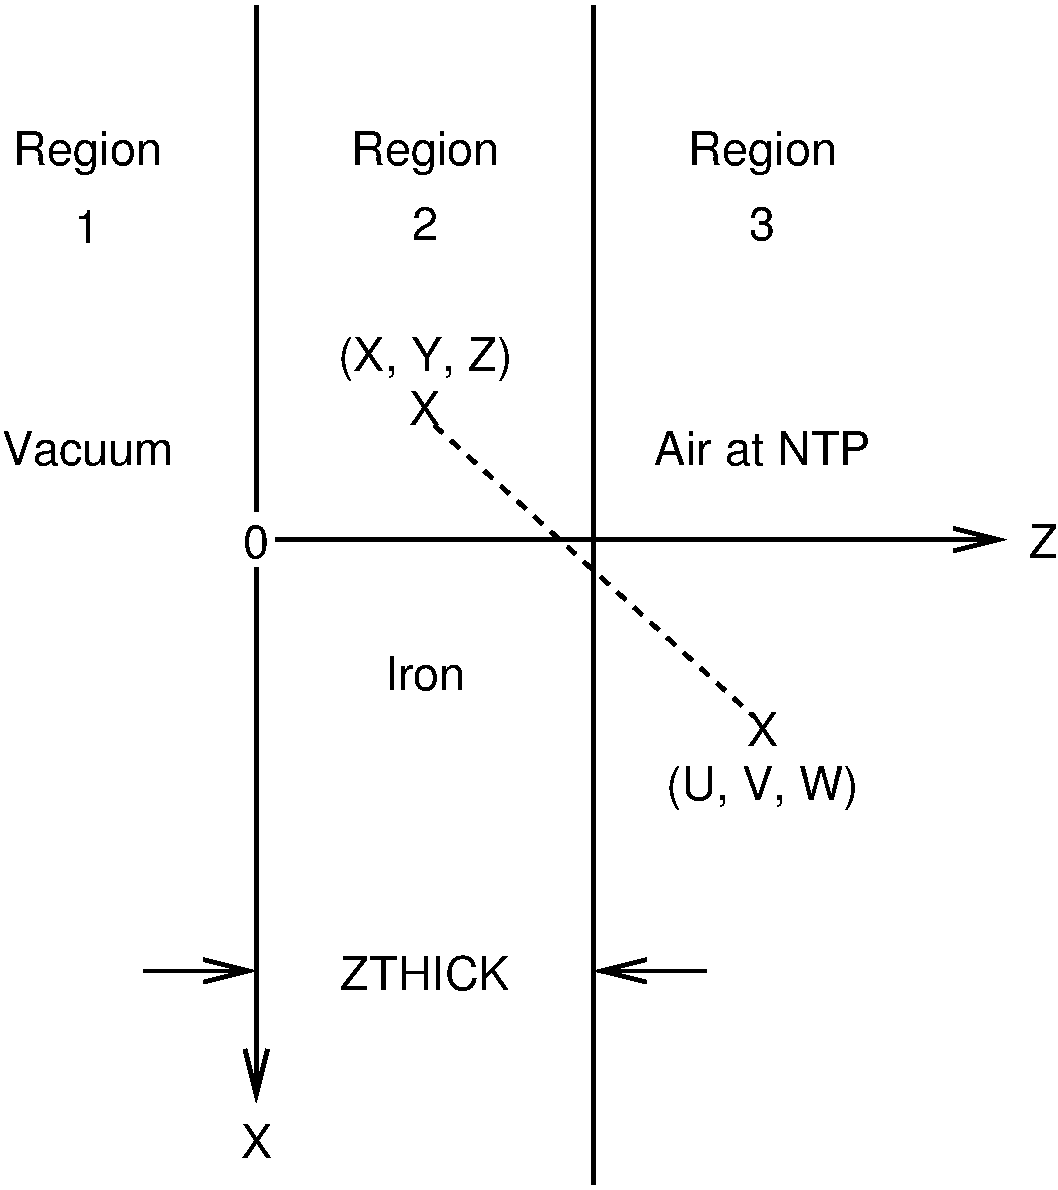
\includegraphics[width=10cm]{figures/3_region_ex}
   \end{center}
   \caption{A 3 region geometry example for HOWFAR.  The Y axis is into the
paper.}
   \label{fig_3_region_ex}
\end{figure}
Consider, as an example of how to write a {\tt HOWFAR} subroutine, the three
region geometry in fig~\ref{fig_3_region_ex}.  A particle is shown in
Region 2 with coordinates (X,Y,Z) and direction cosines (U,V,W).  We will
assume that the slab of thickness {\tt ZTHICK} is semi-infinite (x and
y-directions), and that particles are immediately discarded whenever they
go into Region 1 or Region 3.  The following {\tt HOWFAR} code is then
applicable:
\begin{verbatim} 
     SUBROUTINE HOWFAR;
     COMIN/EPCONT,STACK/;      "common blocks needed in calculations"
     COMMON/GEOM/ZTHICK;       "slab thickness defined in main"
     IF(IR(NP) ~= 2) [IDISC=1; RETURN;]
     IF(W(NP) =  0.0) [RETURN; "particle going parallel to planes"]
     "check forward plane first since shower heading that way"
     "                                       most of the time"
     IF(W(NP) > 0.0) [DELTAZ=(ZTHICK-Z(NP))/W(NP); IRNEXT=3;]
     "otherwise, particle must be heading in backwards direction"
     ELSE [DELTAZ=-Z(NP)/W(NP); IRNEXT=1;]
     "now check with USTEP and reset things if necessary"
     IF(DELTAZ <= USTEP) [USTEP=DELTAZ; IRNEW=IRNEXT;]
     RETURN;  END;
\end{verbatim}
\index{HOWFAR!example}
 
\index{PLAN2P}
\index{\$PLAN2P}
A number of geometry subprograms and their macro equivalents are
distributed with the EGS Code System in order to make it easier to write
{\tt HOWFAR}.  For example, {\tt SUBROUTINE PLAN2P}, or its equivalent macro {\tt
\$PLAN2P}, could have been used in place of several lines above and the
program would have been easier to read.

\index{Bielajew, Alex}
For an advanced discussion of coding {\tt HOWFAR} routines, see Alex Bielajew's
PIRS-341 report ``HOWFAR and HOWNEAR: Geometry Modeling for Monte Carlo
Particle Transport''\cite{Bi95a}.


\subsection{Specifications for HOWNEAR}
\label{hownear}
\index{HOWNEAR!specifications}
\index{\$CALL-HOWNEAR}


As mentioned in section~\ref{hownear_macro}(page~\pageref{hownear_macro}),
for compatibility with previous  EGS4/PRESTA user codes, 
EGSnrc formally requires a macro definition which defaults to:
\begin{verbatim}
REPLACE {$CALL-HOWNEAR(#);} WITH {CALL HOWNEAR({P1},X(NP),Y(NP),Z(NP),IRL);}
\end{verbatim}
where the variable {\tt \#} is {\tt tperp}, the closest distance to
any boundary.  If you are starting from scratch it is easiest to code
{\tt HOWNEAR} as a subroutine.
\index{EGS4}


{\tt SUBROUTINE HOWNEAR} is concerned with the geometry but its job is
somewhat simpler to define than for {\tt SUBROUTINE HOWFAR} since it need
only return one value, namely {\tt tperp}, the distance to the closest
boundary in {\bfseries any} direction.  Unlike {\tt HOWFAR}, {\tt HOWNEAR} passes the
transport parameters parameters to the subroutine as:
\begin{verbatim}
           SUBROUTINE HOWNEAR(tperp, x,y,z, irl);
\end{verbatim}
where \verb+x,y,z+ are the current positions of the particle and \verb+irl+
is its current region.  The rest of the information about the geometry is
passed in whatever {\tt COMMONs} contain the necessary information. In NRCC
user codes and the tutorial codes this is {\tt COMMON/GEOM/;} but it can be
called anything the user wants. 

One simplification is that the routine does not have to handle regions
outside the geometry (as {\tt SUBROUTINE HOWFAR} must in order to have them
discarded).

In complex geometries, the mathematics of {\tt HOWNEAR} can become difficult and
sometimes almost impossible!  If it is easier for the user to compute
some lower bound to the nearest distance, this could be
used in {\tt HOWNEAR}.  In the worst case, one can return \verb+tperp+ as 0.0
in which case the code goes into single scattering mode if using the
exact boundary crossing algorithm.  In fact, this is an easy general way to
turn on single scattering throughout the entire geometry.

The following is an example of a {\tt HOWNEAR} routine for the geometry given
above in section~\ref{howfar} concerning {\tt HOWFAR}.
See also section~\ref{hownear_change} (page~\pageref{hownear_change}).
\begin{verbatim}
     SUBROUTINE HOWNEAR(tperp,X,Y.Z,IRL);
     COMMON/GEOM/ZTHICK; "slab thickness defined in main"
     tperp = min(Z,ZTHICK-Z);
     RETURN;  END;
\end{verbatim}
\index{HOWNEAR}



\subsection{Specifications for AUSGAB}
\label{ausgab}
\index{AUSGAB!specifications}
 
The subroutine {\tt AUSGAB} is called by EGS with the statement:
\begin{verbatim}
      CALL AUSGAB(IARG);
\end{verbatim}
The argument {\tt IARG} indicates the situation under which {\tt AUSGAB}
is being called.  {\tt IARG} can take on 29 values starting from zero
(i.e., {\tt IARG}=0 through {\tt IARG}=28), although only the first
five are called by default in EGSnrc.  The remaining 24 {\tt IARG}
values must be ``switched-on" by means of the array {\tt IAUSFL}.
The value for {\tt IARG} and the corresponding situations are given in
Table~\ref{tab_iausfl_low}.

On occasion one wants to terminate a particle histroy from withing AUSGAB.
To do this cleanly and efficiently set {\tt E(NP) = 0}. One can also set
the weight to zero if you do not want any {\tt EDEP} energy to be scored.

The {\tt IARG} values in table~\ref{tab_iausfl_low} are the ones
generally required in the majority of situations in which EGS is used
to simulate electromagnetic cascade shower development.  In particular,
{\tt IARG}=0 is useful whenever track lengths are being calculated or when
charged particle ionization loss is needed.  Also, as a check on energy
conservation, {\tt EDEP} can be summed in {\tt AUSGAB} for all {\tt IARG}
values less than 5.  The extended {\tt IARG} range allows the user to
extract additional information without making changes to the EGS coding.
To do this we have created the integer flag array, {\tt IAUSFL(J)},
for J=1 through 29.  It takes on values of 1 or 0 depending on whether
{\tt AUSGAB} is called or not, respectively.  For J=1 through 5, which
corresponds to {\tt IARG}=0 through 4, {\tt IAUSFL(J)=1} (default).
In other words, {\tt AUSGAB} is always called for the situations
listed in Table~\ref{tab_iausfl_low}.  For the remaining values of J,
corresponding to {\tt IARG}=5 through 28, {\tt IAUSFL(J)=0} (default).
The value for {\tt IARG} and the corresponding situations for this upper
set of {\tt IARG} values are shown in Table~\ref{tab_iausflg_other}.
\index{IAUSFL}
\index{IARG}
\index{PCUT}
\index{ECUT}
    \begin{table}[hbt]
\index{IAUSFL}
\index{IARG}
\index{PCUT}
\index{ECUT}
    \begin{center}
\caption{Values of {\tt IARG} which are on by default and for which energy is
deposited.}
    \label{tab_iausfl_low}
\vspace*{4mm}
    \begin{tabular}{ c   p{135mm}l  |}
    \hline
    {\tt IARG} & ~~~~~~~~~~~~~~~~~~~~~~~~~~~~~~~~Situation \\
    \hline
0	& Particle is going to be transported by distance TVSTEP.\\
    &\\
1	&Particle is going to be discarded because its energy is below the
cutoff {\tt ECUT} (for charged particles) or {\tt PCUT} (for photons)---but its energy
is larger than the corresponding PEGS cutoff AE or AP, respectively.\\
    &\\
2	& Particle is going to be discarded because its energy is below
both {\tt ECUT} and {\tt AE} (or {\tt PCUT} and {\tt AP}).\\
	&\\
3	& Particle is going to be discarded because the user requested it
(in {\tt HOWFAR} usually or by range rejection).  \\
	&\\
4	&The difference between the energy of the incident particle and
         all of the final products is being deposited locally. This 
         energy is  due to sub-threshold relaxation events.\\
	&\\
\hline
\end{tabular}
\end{center}
\end{table}
\index{IARG} \index{IAUSFL}
\index{AUSGAB} \index{interogating EGSnrc}
    \begin{table}[htbp]
\index{Coster-Kronig electrons}
\index{IARG} \index{IAUSFL}
    \begin{center}
    \caption{Values of {\tt IARG} which are off by default.}
    \label{tab_iausflg_other}
     \vspace*{2mm}
    \begin{tabular}{ c c   p{125mm}l }
    \hline
    {\tt IARG} & {\tt IAUSFL} & ~~~~~~~~~~~~~~~~~~~~~~~~~~~~~~~~Situation \\
    \hline
5&6&  Particle has been transported by distance TVSTEP.\\
&&\\
6&7& A bremsstrahlung interaction is to occur and a call
             to BREMS is about to be made in ELECTR.\\
7&8& Returned to ELECTR after a call to BREMS was made.\\
&&\\
8&9& A Moller interaction is to occur and a call to
             MOLLER is about to be made in ELECTR.\\
9&10& Returned to ELECTR after a call to MOLLER was made.\\
&&\\
10&11&  A Bhabha interaction is to occur and a call to
             BHABHA is about to be made in ELECTR.\\
11&12& Returned to ELECTR after a call to BHABHA was made.\\
&&\\
12&13& An in-flight annihilation of the positron is to
             occur and a call to ANNIH is about to be made
             in ELECTR.\\
13&14& Returned to ELECTR after a call to ANNIH was made.\\
14&15&  A positron has annihilated at rest.\\
&&\\
15&16& A pair production interaction is to occur and a
             call to PAIR is about to be made in PHOTON.\\
16&17& Returned to PHOTON after a call to PAIR was made.\\
&&\\
17&18& A Compton interaction is to occur and a call to
             COMPT is about to be made in PHOTON.\\
18&19& Returned to PHOTON after a call to COMPT was made.\\
&&\\
19&20& A photoelectric interaction is to occur and a call
             to PHOTO is about to be made in PHOTON.\\
20&21& Returned to PHOTON after a call to PHOTO was made
             (assuming {\tt NP} is non-zero).\\
&&\\
21&22& Subroutine UPHI was just entered. Not entered in
all cases now since the sampling is done more efficiently directly in some 
subroutines.\\
22&23& Subroutine UPHI was just exited.\\
&&\\
23&24& A coherent (Rayleigh) interaction is about to occur.\\
24&25& A coherent (Rayleigh) interaction has just occurred.\\
&&\\
25 &26& A fluorescent photon has just been created in RELAX.\\
26 & 27& A Coster-Kronig electron has just been created in RELAX.\\   
27 &28& An Auger electron has just been created in RELAX.\\   
&&\\
28 &29& A positron is about to annihilate at rest.\\   
\hline
\end{tabular}
\end{center}
\end{table}

As an example of how to write an {\tt AUSGAB} subprogram, consider the previous
three region geometry (Fig. \ref{fig_3_region_ex}).  Suppose that we wish to
score (i.e., output on the line printer) only photons that go from Region 2
into Region 3.  The {\tt AUSGAB} subprogram that will accomplish this is given
below.  In this example we print out the stack variables plus {\tt IARG}.  
\index{AUSGAB!example}
\begin{verbatim} 
    SUBROUTINE AUSGAB(IARG);
    COMIN/STACK/;
    "only output information for photons that are discarded"
    "(by the user) in region 3"
    IF(IARG = 3 & IQ(NP) = 0 & IR(NP) =  3) [
        OUTPUT E(NP),X(NP),Y(NP),Z(NP),U(NP),V(NP),W(NP),
          IQ(NP),IR(NP),IARG;  (7G15.7,3I5);]
    RETURN;  END;
\end{verbatim}
The tutorial programs described in
section~\ref{tutorials}(page~\pageref{tutorials}) give examples of various
types of {\tt AUSGAB} routines.

\subsubsection{Checking for STACK overflow}
\index{EGS4} \index{\$MXSTACK} 
\index{STACK overflow} 
Unlike  EGS4, EGSnrc prevents the user from placing
too many particles on the {\tt STACK}. This is implemented via a macro
called {\tt \$CHECK-STACK(\#,\#);} which will terminate the execution if the
stack pointer exceeds {\tt \$MXSTACK}. This check takes some time (not much)
but to optimize the speed of a calculation, one might want to redefine it
as a null macro once one is moving to production runs.   
\begin{verbatim}
      REPLACE {$CHECK-STACK(#,#);} WITH {;}
\end{verbatim}
Even if the above macro is nulled out, EGSnrc continues to verify that
there is adequate space on the stack whenever radiative splitting is being
used.
\index{\$CHECK-STACK}

\subsubsection{Status of the STACK at various AUSGAB calls}
\label{stack_status}
\index{STACK!order}
\index{EGS4}
In EGS4, the general rule was that after an interaction, the lowest energy
particle was always on the top of the {\tt STACK}. This general rule has
been relaxed in EGSnrc, partially because of the new physics, and partially
because memory is not as expensive as it once was.

\index{bound Compton scattering}
With the addition of relaxation events in EGSnrc, the possibilities
about what is on the stack after various events has become more complex
than in EGS4. For example, after a Compton scattering event in {\tt
EGS4}
({\tt IARG}=18), one could count on the {\tt STACK} having one more particle on it
compared to just before the call ({\tt IARG}=17). In EGSnrc, when bound compton
is being simulated, this is no longer the case.  Firstly, because of the
rejection techniques used to determine if the event actually took place
(see section~\ref{compton},page~\pageref{compton}) it is possible that only the
original photon is on the stack. At the opposite extreme, the scattered
photon and electron may be on the {\tt STACK} along with 2 or 3 relaxation
particles (fluorescent x-rays, Auger electrons, Coster-Kronig electrons).
Another complication occurs if Russian Roulette is being used since in this
case there can be events in which there is nothing left on the {\tt STACK} after
the event (e.g. after a pair event where the particles are discarded).
To help sort out these situations, EGSnrc has the variable {\tt
NPold} in {\tt COMIN STACK} which points to the position on the stack of the initiating particle
(the photon prior to Compton scattering, Rayleigh scattering, pair
production, photo-electric event or the electron prior to Moller scattering
or a bremsstrahlung event, etc).

Another change with EGSnrc is that the ordering of the resultant particles
is not rigorously set as lowest to highest energy.  This saves computing
time and with the reduced cost of memory, the issue of the size of the
{\tt STACK} is not so critical, at least not for low energy simulations ($<$100
MeV).  However, for high-energy simulations this may cause problems. To
overcome these the user code could define the macros {\tt
\$PARTICLE-SELECTION-MOLLER;} (where {\tt MOLLER} can be any interaction)
to sort the stack by energy after whatever interactions needed it. These
macros are by default null macros, but they are placed immediately after
the call to each subroutine which samples a type of event.
\index{\$PARTICLE-SELECTION-}

The ordering on the {\tt STACK} is summarized in the following.  Note that
the introduction of electron impact ionization and relaxation after other
than the photoelectric events has led to significant changes.
\begin{description}

\index{photoelectric interactions}
\item[Photoelectric] {\tt NPold} points at the photoelectron unless the initial
photon energy is $<$1~keV in which case there is an error message and an
electron with the photon's energy is created. Another exception occurs if
the photon's energy is less than the N-shell binding (which can only occur
for Z$\ge$96), in which case {\tt EDEP} is set to the photon's energy and a
photon of energy 0.0 is left at {\tt NPold}.  For normal events, the
particles from \verb^NPold+1^ to {\tt NP} are due to relaxation events.  If
internal Russian Roulette is being played (see section~\ref{rusrou}), it is
possible for {\tt NP} to be {\tt NPOLD - 1} after the event where there is
no fluorescent photon and all the resulting electrons are killed by the
Russian Roulette.  \index{Russian Roulette}

\index{bound Compton scattering}
\index{Compton scattering}
\item[Compton scattering] For Klein-Nishina modelling, the scattered photon and
electron are in {\tt NPold} and \verb^NPold+1 = NP^ respectively (i.e. the energy is not
ordered).  When bound compton scattering is
being modelled, there are several possibilities. At one extreme, since a
rejection technique is used, the scattering may not occur. In this case,
\verb^NPold = NP^.  If the scattering occurs, then the scattered photon and
compton electron are in \verb^NPold^ and \verb^NPold+1^, as in the Klein-Nishina case. If
there are any relaxation particles (i.e. \verb^NP > NPold+1^), they are found
in \verb^NPold+2^ to \verb^NP^.  There is a slight complication if the internal Russian
Roulette is being used (see section~\ref{rusrou}) 
since, if all the electrons disappear because of Russian Roulette, then
NPold=NP. To distinguish these two cases, the flag {\tt i\_survived\_RR}
can be used. It has a value 0 for the case of an unbound interaction being
rejected and has a value $>$ 0 if the interaction occurred and all
secondaries were eliminated by Russian Roulette.
\index{i\_survived\_RR}

\index{pair production}
\item[Pair Production] For pair production the electron and positron are
in {\tt NPold} and\\ \verb^NPold+1 = NP^ with the lower energy particle on the
top of the {\tt STACK} (at \verb^NP^). If internal Russian Roulette kills
the electron - positron pair, then,
\verb^NP = NPold-1^ unless this would leave \verb^NP = 0^, in which a
zero energy photon is placed on the {\tt STACK} with \verb^NP = 1^.

\index{Rayleigh scattering}
\item[Rayleigh scattering] In this case, the photon is still at
\verb^NPold^.

\index{bremsstrahlung!production}
\index{bremsstrahlung!splitting}
\item[Brem production] In this case, the resulting electron is
always at \verb^NPold^ and the photon is on top of the {\tt STACK} at \verb^NPold+1^, i.e. the
lowest energy particle is not necessarily on the top of the STACK. When
bremsstrahlung splitting is being used. The photons are between
\verb^NPold+1^ and
\verb^NP^. Note that they are not ordered by energy.

\index{Moller scattering}
\item[Moller scatter] There are 3 possible situations after a call to the
Moller routine. If a `standard' Moller scattering has occured, the
resulting, lower energy electron is in \verb^NPold+1 = NP^ and the rpimary
is at \verb^NPold^. It is possible
that the incident electron's energy is below the threshold for creating a
secondary and the return is with \verb^NP^=\verb^NPold^. If this call to
Moller led to an electron impact ionization, the priumary electron will be
at \verb^NPold^ and there may be relaxation events
from  \verb^NPold+1^ to \verb^NP^ although in the extreme case of all energy
deposition below threshold \verb^NP^=\verb^NPold^ and there is only the
primary electron.

\index{Bhabha scattering}
\item[Bhabha scatter] The resulting positron and electron are at
\verb^NPold^ and
\verb^NPold+1^, ordered by their energies.

\index{annihilation}
\item[Annihilation] The two resulting photons are at \verb^NPold^ and
\verb^NPold+1^
unless bremsstrahlung splitting is being used in which case the photons go
from \verb^NPold^ to \verb^N^P. The particle energies are not ordered.

\index{relaxation}
\item[Relaxation] There can be separate calls to AUSGAB after the
individual relaxation events (fluorescent photon, Coster-Kronig or Auger
electrons) but note that after the complete relaxation there may also be
ASUGAB calls post Moller, photoelectric and Compton and one should avoid
double counting.

\end{description}

\subsection{Terminating particle histories}
\label{termination}
\index{terminating particle history}
\index{weight}
\index{IDISC}
\index{WT=0.0}
The standard method to terminate a history is by setting
IDISC to a non-zero value in HOWFAR (see section~\ref{howfar},
page~\pageref{howfar}).  Another method is to set the weight of
a particle to 0.0, usually in AUSGAB under some conditions (e.g. when
doing Russian Roulette).  This technique is used in EGS4 by checking the
weight of a particle as it enters HOWFAR and setting IDISC non-zero if the
weight is zero.  This is somewhat wasteful since it means that various
parameters are calculated for this particle, despite the fact that it
is going to be discarded. In particular, we found that if we were also
using the standard photon forcing macro we got into an infinite loop.
This could have been corrected by re-coding the macro to handle weight
0.0 particles differently, but it was decided that we could save more
time by adding a test at the start of the new electron or new photon loops
whereby a particle is discarded immediately via the {\tt
USER-PHOTON-DISCARD} or {\tt USER-ELECTRON-DISCARD} if the weight is 0.0.
This generates a call to AUSGAB with {\tt IARG = 3}. Positrons discarded
this way do not create annihilation photons. Note that {\tt
ELKE} is not available with this call since it is assumed the particle
is being thrown away.  One should still have HOWFAR set {\tt IDISC = 1}
when the weight is 0.0, especially if the weight is set to zero for a
particle which is not new.


\subsection{Random number generators}
\label{rngs}
\index{random number generators}
\index{RANLUX}
\index{RANMAR}
\index{luxury level}

\index{EGS4}
EGSnrc is supplied with two random number generators, RANLUX
and RANMAR.  RANMAR is the generator used with EGS4 in the unix
distributions\cite{MZ91,Ma90a} and although it is known to fail certain
theoretical tests, we have no experience of it causing problems.
The RANLUX generator\cite{La94,Ja94}, which is treated as the default
generator with EGSnrc, is a similar sort of generator which comes
with a variety of ``luxury levels'', from 0 to 4 and a period of
greater than 10$^{165}$.  According to James, RANMAR has a
quality somewhere between luxury level 1 and 2 of RANLUX
and we have found
that it gives incorrect answers in some practical EGSnrc calculations
with luxury level 0. However, with luxury level 1 or higher we have
seen no problems.  We have utilized RANLUX as the default rng because
it allows explicit testing with higher quality sequences if there are
ever any doubts.

Both random number generators offer several important features. Firstly,
they are completely portable, producing the same sequences on different
machines, although RANMAR occasionally gets slightly out of sequence and
sometimes optimizers on a given machine will cause the sequences to differ.
We have not seen this behaviour with RANLUX.  An even more important
feature is that either generator can be initialized and guaranteed to
produce a random number sequence which is independent from other sequences.
This is very useful for doing runs in parallel on multiple machines.
\index{parallel processing}
 

The default generator is defined in {\tt
\$HEN\_HOUSE/specs/all\_common.spec} by the statement {\tt RANDOM =
\$(EGS\_SOURCEDIR)ranlux}. This can be changed to {\tt ranmar} or,
for individual user codes, it can be changed by adding the statement
{\tt RANDOM = \$(EGS\_SOURCEDIR)ranmar} to the {\tt user\_code.make}
file, somewhere before the {\tt SOURCES =} statement (if it exists).
See Report PIRS-877 for further information about {\tt make} files in
the EGSnrcMP environment\cite{Ka03}.

These files provide the following macros which the user is free to use in
their user code:
\begin{verbatim}
        ;COMIN/RANDOM/;
        $RANDOMSET#;
        $DEFAULT-LL   (1 by default)
        $RNG-INITIALISATION;    (which is only needed optionally)
        $INITIALIZE RNG USING # AND #; (a more useful version of the above)
        $STORE RNG STATE ON UNIT #;
        $PUT RNG STATE ON UNIT #;
        $RETRIEVE RNG STATE FROM UNIT #;
        $SHOW-RNG-STATE(#);
        $PRINT-RNG-STATE(#,#);
        $RNG-INPUTS(#,#,#,#);  (uses GET_INPUTS routine)
\end{verbatim}
\index{\$DEFAULT-LL}
To generate a random number, say {\tt RNUMBER}, include:
\begin{verbatim}
          $RANDOMSET RNUMBER;
\end{verbatim}
Wherever the user needs to use {\tt \$RANDOMSET\#;}, they must ensure
{\tt COMIN/RANDOM/} is present.
\index{RANDOM}
\index{macro!\$RANDOMSET}
\index{\$RANDOMSET}
If the user is happy with luxury level 1 and the same sequence for each
calculation, the RANLUX generator is self-initializing. However, to use
other luxury levels or other sequences, the user code should include
a statement of the type:
\begin{verbatim}
         $INITIALIZE RNG USING luxury_level AND iseed;
\end{verbatim}
where {\tt luxury\_level} is an integer between 0 and 4 and {\tt iseed}
is any positive integer (and if left 0, a default of {\tt 314159265} is used).
\index{\$INITIALIZE RNG USING}

For a standard production run of one of the NRC user codes (CAVRZnrc for
$^{60}$Co photons incident on a thimble chamber with splitting of 130) we
get the timing results shown in table~\ref{tab_ll_times}, although these
values are revised from the pre-2003 printings and depend on the details of
any simulation.  Given the iproblems encountered using luxury level 0, 
luxury level 1 has been
adopted as the default with EGSnrc. However, given a new coding of RANMAR
to generate groups of random numbers using a function call, we find that
RANMAR is faster (by 5\% say overall).  The penalty ifor using higher
RANLUX luxury levels becomes increasingly more
important at higher luxury levels and a user may want to verify that for
their simulations, use of the higher level makes no difference. We would
appreciate being informed of any cases found where luxury level 1 was not
adequate.
\index{random number generators!timing}
\index{luxury level!timing}
\begin{table}[htb]
\begin{center}
\caption{Calculation times for runs with CAVRZnrc for the same calculations
along with estimates of the time taken by the random number generator at
different luxury levels.  The results for luxury level 0 are different when
high precision is obtained.\vspace{3mm}
\label{tab_ll_times}
}
\begin{tabular}{ |c c c c |}
\hline
Luxury level & total CPU time  & \multicolumn{2}{c|}{time taken by RANLUX} \\
             &  s &  s  & \%\\
\hline
&&&\\
0	&194	& 24 & 12\% \\
1	&210	& 39 & 18\% \\
2	&240	& 68 & 28\% \\
3	&315	& 142  &45\% \\
4	&415	& 242  &58\% \\
&&&\\
\hline
    \end{tabular}
    \end{center}
    \end{table}


When using the RANMAR generator, the initialisation looks like:
\begin{verbatim}
         $INITIALIZE RNG USING IXX AND JXX;
\end{verbatim}
where {\tt IXX} and {\tt JXX} are two integers seeds with:
\cen{{\tt  0$<$ IXX$<=$31328} and {\tt 0$<$JXX$<=$30081}}

The other macros are for use when saving the state of a random number
generator to disk and possibly restarting a run or other book keeping tasks.

There are two files available for use in codes doing correlated
sampling.  These files are:
\begin{verbatim}
       ranlux.correlations    or      ranmar.corrrelations
\end{verbatim}
These files define the macros:
\begin{verbatim}
        $STORE-RNG(#);
        $RESET-RNG(#);
\end{verbatim}
which store and reset an arbitrary number of random number states ($\le${\tt
\$MXRNGDIM} which is 5 by default).

Note: because of how the RANLUX generator is implemented, it is essential
that any redefined {\tt COMIN/RANDOM} must include an integer variable
called {\tt rng\_seed}. This variable is initialized to 999999 in {\tt
egs\_set\_default} which replaces {\tt BLOCK DATA} in the EGSnrcMP
environment\cite{Ka03}.
\index{RANDOM} \index{COMMON!RANDOM}
\index{random number generators}
\index{RANLUX}
\index{RANMAR}
\index{\$STORE-RNG}
\index{\$RESET-RNG}

\subsection{Summary of transport parameter}
\label{param_options}
\index{transport parameter summary}
\index{cross section options}


In many cases transport parameters and cross section options will be 
controlled via an input file that uses a {\tt option = value} format 
(\eg~all RZ user codes, all C++ codes). The following provides a summary 
of the options available along with possible settings.

%%%%%%%%%%%%%%%%%%%%%%%%%%%%%%%%%%%%%%%%%%%%%%%%%%%%%%%%%%%%%%%%%%%%%%%%%%%%%%%
%
%  EGSnrc manual: transport parameters
%  Copyright (C) 2015 National Research Council Canada
%
%  This file is part of EGSnrc.
%
%  EGSnrc is free software: you can redistribute it and/or modify it under
%  the terms of the GNU Affero General Public License as published by the
%  Free Software Foundation, either version 3 of the License, or (at your
%  option) any later version.
%
%  EGSnrc is distributed in the hope that it will be useful, but WITHOUT ANY
%  WARRANTY; without even the implied warranty of MERCHANTABILITY or FITNESS
%  FOR A PARTICULAR PURPOSE.  See the GNU Affero General Public License for
%  more details.
%
%  You should have received a copy of the GNU Affero General Public License
%  along with EGSnrc. If not, see <http://www.gnu.org/licenses/>.
%
%%%%%%%%%%%%%%%%%%%%%%%%%%%%%%%%%%%%%%%%%%%%%%%%%%%%%%%%%%%%%%%%%%%%%%%%%%%%%%%
%
%  Author:          Frederic Tessier, 2011
%
%  Contributors:
%
%%%%%%%%%%%%%%%%%%%%%%%%%%%%%%%%%%%%%%%%%%%%%%%%%%%%%%%%%%%%%%%%%%%%%%%%%%%%%%%


\index{ECUT}
\begin{verbatim}
       Global ECUT=     Global (in all regions) electron transport cut
                        off energy (in MeV). If this input is missing,
                        AE(medium) will be used.
                        [ ECUT ]
\end{verbatim}
\index{PCUT}
\begin{verbatim}
       Global PCUT=     Global (in all regions) photon transport cut
                        off energy (in MeV). If this input is missing,
                        AP(medium) will be used.
                        [ PCUT ]
\end{verbatim}
\index{SMAX}
\begin{verbatim}
       Global SMAX=     Global (in all regions) maximum step-size
                        restriction for electron transport (in cm).
                        If missing, no geometrical step-size restrictions
                        will be employed. Note that if you use the default
                        EGSnrc electron-step algorithm, no SMAX-restriction
                        is necessary. Option is useful for transport in low
                        density materials (air) when PRESTA behaviour is
                        turned on (see below)
                        [ SMAXIR ]
\end{verbatim}
\index{ESTEPE}
\begin{verbatim}
       ESTEPE=          Maximum fractional energy loss per step.
                        Note that this is a global option only, no
                        region-by-region setting is possible. If missing,
                        the default is 0.25 (25%).
                        [ ESTEPE ]
\end{verbatim}
\index{XImax}
\begin{verbatim}
       XImax=           Maximum first elastic scattering moment per step.
                        Default is 0.5, NEVER use value greater than 1 as
                        this is beyond the range of MS data available.
                        [ XIMAX ]
\end{verbatim}
\index{boundary crossing algorithm}
\index{bca\_algorithm}
\index{exact\_bca}
\index{transport\_algorithm}
\begin{verbatim}
       Boundary crossing algorithm= EXACT (default), PRESTA-I
                        There are two selections possible: EXACT means
                        the algorithm will cross boundaries in a single
                        scattering (SS) mode, the distance from a boundary
                        at which the transition to SS mode is made is
                        determined by 'Skin depth for BCA' (see below).
                        The second option is PRESTA-I, if selected boundaries
                        will be crossed a la PRESTA, i.e. with lateral
                        correlations turned off and MS forced at boundaries.
                        Default is EXACT.
                        [ bca_algorithm, exact_bca ]
\end{verbatim}
\index{skin depth for BCA}\index{exact\_bca}
\index{skindepth\_for\_bca}
\begin{verbatim}
       Skin depth for BCA=
                        Determines the distance from a boundary (in elastic
                        MFP) at which the algorithm will go into single
                        scattering mode (if EXACT boundary crossing) or
                        switch off lateral correlations (if PRESTA-I boundary
                        crossing). Default value is 3 for EXACT or
                        exp(BLCMIN)/BLCMIN for PRESTA-I (see the PRESTA paper
                        for a definition of BLCMIN). Note that if you choose
                        EXACT boundary crossing and set Skin depth for BCA
                        to a very large number (e.g. 1e10), the entire
                        calculation will be in single-scattering mode. If you
                        choose PRESTA-I boundary crossing and make Skin depth
                        for BCA large, you will get default EGS4 behaviour
                        (no PRESTA).
                        [ skindepth_for_bca ]
\end{verbatim}
\index{electron step algorithm}
\begin{verbatim}
       Electron-step algorithm= PRESTA-II (default), PRESTA-I (legacy)
                        Determines the algorithm used to take into account
                        lateral and longitudinal correlations in a
                        condensed history step.
                        [ transport_algorithm ]
\end{verbatim}
\index{spin effects}
\index{spin\_effects}
\begin{verbatim}
       Spin effects=    Off, On (default)
                        Turns off/on spin effects for electron elastic
                        scattering. Spin On is ABSOLUTELY necessary for
                        good backscattering calculations. Will make a
                        difference even in `well conditioned' situations
                        (e.g. depth dose curves for RTP energy range
                        electrons).
                        [ spin_effects ]
\end{verbatim}
\index{brems angular sampling}
\index{IBRDST}
\begin{verbatim}
       Brems angular sampling= Simple, KM (default)
                        If Simple, use only the leading term of the Koch-Motz
                        distribution to determine the emission angle of
                        bremsstrahlung photons. If KM, complete
                        modified Koch-Motz 2BS is used (modifications
                        concern proper handling of kinematics at low energies,
                        makes 2BS almost the same as 2BN at low energies).
                        [ IBRDST ]
\end{verbatim}
\index{brems cross section}
\index{ibr\_nist}
\begin{verbatim}
       Brems cross sections= BH (default), NIST, NRC
                        If BH is selected, the Bethe-Heitler bremsstrahlung
                        cross sections (Coulomb corrected above 50 MeV)
                        will be used. If NIST is selected, the NIST brems
                        cross section data base (which is the basis for
                        the ICRU radiative stopping powers) will be employed.
                        Differences are negligible for E > ,say, 10 MeV,
                        but significant in the keV energy range. If NRC is
                        selected, the NRC brems cross-section data base will
                        be used, which is a version of the NIST data base
                        with corrected electron-electron brems contributions
                        (corrections to the NIST data is typically only
                        significant for low values of the atomic number Z
                        and for k/T < 0.005).
                        [ ibr_nist ]
\end{verbatim}
\index{triplet production}
\index{itriplet}
\begin{verbatim}
       Triplet production= On or Off (default).  Turns on/off simulation
                        of triplet production.  If On, then Borsellino's
                        first Born approximation is used to sample triplet
                        events based on the triplet cross-section data.
                        [ itriplet ]
\end{verbatim}
\index{bound Compton scattering}
\index{IBCMP}
\begin{verbatim}
       Bound Compton scattering=  On, Off, Simple or norej (default)
                        If Off, Compton scattering will be treated with
                        Klein-Nishina, with On Compton scattering is
                        treated in the Impulse approximation.
                        With Simple, the impulse approximation incoherent
                        scattering function will be used (i.e., no Doppler
                        broadenning). With norej the actual total bound
                        Compton cross section is used and there are no
                        rejections at run time.
                        Make sure to turn on for low energy applications,
                        not necessary above, say, 1 MeV.
                        [ IBCMP ]
\end{verbatim}
\index{radiative Compton corrections}
\index{radc\_flag}
\begin{verbatim}
       Radiative Compton corrections= On or Off (default). If On, then
                        include radiative corrections for Compton scattering.
                        Equations are based on original Brown & Feynman
                        equations (Phys. Rev. 85, p 231--1952).  Requires
                        a change to the user codes Makefile to include
                        $(EGS_SOURCEDIR)rad_compton1.mortran in the
                        SOURCES (just before
                        $(EGS_SOURCEDIR)get_inputs.mortran).
                        [ radc_flag ]
\end{verbatim}
\index{electron impact ionization}
\index{eii\_flag}
\begin{verbatim}
       Electron Impact Ionization= Off (default), On, casnati, kolbenstvedt,
                        gryzinski or penelope.  If set to On or ik, then
                        use Kawrakow's theory to derive EII cross-sections.
                        If set to casnati, then use the cross-sections of
                        Casnati (from file $HEN_HOUSE/data/eii_casnati.data).
                        Similar for kolbenstvedt, gryzinski and penelope.
                        This is only of interest in kV X-ray calculations.
                        Note that the user can supply their own EII
                        cross-section data as well. The requirement is that
                        the file eii_suffix.data exists in the $HEN_HOUSE/data
                        directory, where suffix is the name specified.
                        Entry is case-sensitive except for Off, On or ik.
                        [ eii_flag, eii_xfile ]
\end{verbatim}
\index{pair angular sampling}
\index{IPRDST}
\begin{verbatim}
       Pair angular sampling= Off, Simple (default), KM.
                        If off, pairs are set in motion at an angle m/E
                        relative to the photon direction (m is electron rest
                        energy, E the photon energy). Simple turns on
                        the leading term of the angular distribution
                        (this is sufficient for most applications),
                        KM (comes from Koch and Motz) turns on using 2BS
                        from the article by Koch and Motz.
                        Default is Simple, make sure you always use
                        Simple or KM
                        [ IPRDST ]
\end{verbatim}
\index{pair cross sections}
\index{pair\_nrc}
\begin{verbatim}
       Pair cross sections= BH (default) or NRC.  If set to BH, then use
                        Bethe-Heitler pair production cross-sections.  If set
                        to NRC, then use NRC pair production cross-sections
                        (in file $HEN_HOUSE/data/pair_nrc1.data).  Only
                        of interest at low energies, where the NRC cross-
                        sections take into account the asymmetry in the
                        positron-electron energy distribution.
                        [ pair_nrc ]
\end{verbatim}
\index{photon cross sections}
\index{photon\_xsections}
\begin{verbatim}
       Photon cross sections= Photon cross-section data.  Current options are
                        si (Storm-Israel--the default), epdl (Evaluated Photon
                        Data Library), and xcom.  Allows the user to use photon
                        cross-sections other than the default PEGS4 (Storm-
                        Israel) values.  Note that the user can supply their
                        own cross-section data as well.  The requirement is
                        that the files
                        photon_xsections_photo.data,
                        photon_xsections_pair.data,
                        photon_xsections_triplet.data, and
                        photon_xsections_rayleigh.data exist in the
                        $HEN_HOUSE/data directory, where photon_xsections
                        is the name specified.
                        Entry is case-sensitive except for the pegs4 option.
                        [ photon_xsections ]
\end{verbatim}
\index{photon cross sections!output}
\index{xsec\_out}
\begin{verbatim}
       Photon cross-sections output= Off (default) or On.  If On, then
                        a file $EGS_HOME/user_code/inputfile.xsections is
                        output containing photon cross-section data used.
                        [ xsec_out ]
\end{verbatim}
\index{compton cross sections}
\index{comp\_xsections}
\begin{verbatim}
       Compton cross sections= Bound Compton cross-section data.  User-
                        supplied bound Compton cross-sections in the file
                        $HEN_HOUSE/data/comp_xsections_compton.data, where
                        comp_xsections is the name supplied for this input.
                        This is only used if Bound Compton scattering= Simple
                        and is not available on a region-by-region basis
                        (see below).  The default file (ie in the absence
                        of any user-supplied data) is compton_sigma.data.
                        [ comp_xsections ]
\end{verbatim}
\index{Rayleigh scattering}
\index{Rayleigh scattering!custom form factors}
\index{IRAYLR}
\begin{verbatim}
       Rayleigh scattering= Off, On (default), custom
                        If On, turns on coherent (Rayleigh) scattering.
                        Default is On. Should be turned on for low energy
                        applications. If custom, user must provide media names
                        and form factor files for each desired medium. The
                        rest of the media use the default atomic form factors.
                        Not set to On by default for historical reasons since
                        a PEGS4 data set is not required anymore.
                        [ IRAYLR ]
\end{verbatim}
\index{iray\_ff\_media}
\begin{verbatim}
       ff media names = A list of media names (must match media found in
                        PEGS4 data file) for which the user is going to
                        provide custom Rayleigh form factor data.
                        [ iray_ff_media($MXMED) ]
\end{verbatim}
\index{iray\_ff\_file}
\begin{verbatim}
       ff file names = A list of names of files containing the Rayleigh
                       form factor data for the media specified by
                       the ff media names = input above.  Full directory
                       paths must be given for all files, and for each medium
                       specified, iray_ff_media(i), there must be a
                       corresponding file name, iray_ff_file(i).  For
                       example files, see the directory
                       $HEN_HOUSE/data/molecular_form_factors.
                       [ iray_ff_file($MXMED) ]
\end{verbatim}
\index{photonuclear attenuation}
\index{IPHOTONUCR}
\begin{verbatim}
       Photonuclear attenuation= Off (default) or On
                        If On, models the photonuclear effect. Current
                        implementation is crude. Available on a
                        region-by-region basis (see below)
                        [ IPHOTONUCR ]
\end{verbatim}
\index{photonuclear cross sections}
\index{photonuc\_xsections}
\begin{verbatim}
       Photonuclear cross sections= Total photonuclear cross sections. User-
                        supplied total photonuclear cross-sections in
                        $HEN_HOUSE/data/photonuc_xsections_photonuc.data,
                        where photonuc_xsections is the name supplied for
                        this input (case sensitive). In the absence of
                        any user-supplied data, or if photonuc_xsections
                        is set to 'default', the default file is
                        iaea_photonuc.data.
                        [ photonuc_xsections ]
\end{verbatim}
\index{photoelectron angular sampling}
\index{IPHTER}
\begin{verbatim}
       Photoelectron angular sampling= Off or On (default)
                        If Off, photo-electrons get the direction of the
                        `mother' photon, with On, Sauter's formula is
                        used (which is, strictly speaking, valid only for
                        K-shell photo-absorption).
                        If the user has a better approach, replace the macro
                            $SELECT-PHOTOELECTRON-DIRECTION;
                        The only application encountered where this option
                        made a small difference was a big ion chamber
                        (cavity size comparable with electron range)
                        with high-Z walls in a low energy photon beam.
                        [ IPHTER ]
\end{verbatim}
\index{atomic relaxations}
\index{IEDGFL}
\begin{verbatim}
       Atomic relaxations= Off, On, eadl (default), simple
                        On defaults to eadl.
                        When simulating atomic relaxations:
                        - In photo-electric absorption events, the element
                          (if material is mixture) and the shell the photon
                          is interacting with are sampled from the appropriate
                          cross sections
                        - Shell vacancies created in photoelectric,
                          compton and electron impact ionization events
                          are relaxed via emission of fluorescent X-Rays,
                          Auger and Koster-Cronig electrons.
                          The eadl option features a more accurate treatment
                          of relaxation events and uses binding energies
                          consistent with those in of the photon cross sections
                          used in the simulation.  If using mcdf-xcom or
                          mcdf-epdl photon cross sections, you cannot use
                          the simple option and this will automatically get
                          reset to eadl. Make sure to use eadl or simple for
                          low energy applications.
                          [ IEDGFL ]
\end{verbatim}

\noindent
Atomic relaxations, Rayleigh scattering, Photoelectron angular sampling,
Bound Compton scattering and photonuclear effect
can also be turned On/Off on a region-by-region basis. An example for
Atomic relaxations on a region-by-region basis is:

\begin{verbatim}
       Atomic relaxations= On in Regions   or
       Atomic relaxations= Off in regions
\end{verbatim}

Then define the regions in which you want
the feature to be turned on:

\begin{verbatim}
       Bound Compton start region=
       Bound Compton stop region=
                or
       Rayleigh start region=
       Rayleigh stop region=
                or
       Relaxations start region=
       Relaxations stop region=
                or
       PE sampling start region=
       PE sampling stop region=
\end{verbatim}
each followed by a list of one or more
start and stop regions separated by commas.
Example:
\begin{verbatim}
        Atomic relaxations= On in Regions
        Relaxations start region=  1, 40
        Relaxations stop region=  10, 99
\end{verbatim}
will first turn off relaxations everywhere and
then turn on in regions 1-10 and 40-99.
Note that the input is checked against minimum
and maximum region numbers and ignored if
\verb+start region < 1+ or \verb+stop_region > $MXREG+ or
\verb+start region > stop region+.

\verb+ECUT+, \verb+PCUT+ and \verb+SMAX+ can also be set on a
region-by-region basis. To do so, include in the input file
\begin{verbatim}
         Set XXXX=              f_value1, f_value2, ...
         Set XXXX start region= i_value1, i_value2, ...
         Set XXXX stop region=  j_value1, j_value2, ...
\end{verbatim}
where \verb+XXXX+ is \verb+ECUT+, \verb+PCUT+ or \verb+SMAX+,
\verb+f_value1+, \verb+f_value2+,...
are the desired values for \verb+XXXX+ and \verb+i_value_i+ and
\verb+j_value_i+ are the start and stop regions.


\subsection{Variance Reduction Options}
\label{VRO}
\index{variance reduction}
Three forms of variance reduction techniques have been implemented directly
into the EGSnrc system in order to allow for more efficient calculations.
With EGS4 user codes they had to be implemented via calls to {\tt
AUSGAB} or
other means, and this led to inefficiencies.  In all three cases, if the
user does nothing to turn on these options explicitly, then they are NOT
used.
\index{EGS4}

\subsubsection{Range rejection}
\label{range_rejection}

\index{range rejection}
\index{variance reduction}
\index{variance reduction!range rejection}
\index{E\_RANGE}
Within EGSnrc the range of the electron is available at every step. This is
not the true range, but the range determined by:
\[ {\tt E\_RANGE} = \int_{E_{min}}^E \frac{dE^\prime}{L(E^\prime,AE)}\]
where $L(E^\prime,AE)$ is the restricted stopping power for a given value
of AE and $E_{min}$ is the lowest energy for which PEGS4 produces a
stopping power (this is somewhat less than AE, but not much).
The value of {\tt E\_RANGE} is an
upper limit on the distance an electron can travel in the simulation
because discrete events may shorten the pathlength.

\index{\$RANGE-DISCARD}
\index{macro!\$RANGE-DISCARD}
Range rejection is implemented by a macro {\tt \$RANGE-DISCARD} checks
the electron range against the distance to the nearest boundary on
every step. The history is terminated whenever the range is shorter than
the distance to the boundary and if requested by the user.  Since the
range and distance are calculated for other purposes, this check is
very fast and can save a large amount of time, especially in large
regions. Since this is a user controlled discard, it goes via the {\tt
USER-ELECTRON-DISCARD}, generating and {\tt {\tt IARG} = 3}   call to {\tt
AUSGAB}.
\index{USER-ELECTRON-DISCARD}   \index{AUSGAB}

This technique
does involve an approximation since the electron could emit a
brem photon which could escape the region, even if the electron
itself could not.  To control the extent of this approximation, the range
rejection is done only if the electron's energy is below an energy
threshold which can be set for every region, viz {\tt e\_max\_rr}. By
judicial choice of this value, the approximation can be made very accurate
while still obtaining very significant gains in efficiency (see
ref~\cite{Ro95} for a detailed discussion, where the parameter {\tt ESAVE}
in that paper is equivalent to {\tt e\_max\_rr} here).  

Range rejection is implemented on a regional basis by setting the flags
{\tt i\_do\_rr(irl)} to 1 for all regions {\tt irl} for which range
rejection is required and by assigning values to the array {\tt
e\_max\_rr(irl)}. Note that if {\tt e\_max\_rr(irl)} is not assigned a value,
its default value of 0.0 effectively turns off range rejection, even
if {\tt i\_do\_rr(irl)} value is 1.  Both arrays are in {\tt
COMIN/EGS-VARIANCE-REDUCTION}. They need be set before the first
call to {\tt SHOWER}.  Note that {\tt e\_max\_rr(irl)} refers to the
electrons total energy (i.e. includes the rest mass, as does {\tt ECUT}).
\index{EGS-VARIANCE-REDUCTION} \index{e\_max\_rr}
\index{i\_do\_rr} \index{range rejection}

The user is also free to implement other, possibly more efficient forms of
range rejection. This is done by defining the macro {\tt
\$USER-RANGE-DISCARD} which is called immediately after the above macro
since in general, the macro {\tt \$RANGE-DISCARD} executes very quickly
and can avoid use of the user's, presumably more time consuming range
rejection.  An example of {\tt
\$USER-RANGE-DISCARD} is given in CAVRZnrc where range rejection is done on
any particle which cannot reach the region where the dose is required. This
can terminate many histories earlier than {\tt \$RANGE-DISCARD} because it
tests against getting to the region of interest as opposed to just getting
out of the local region.  However, it requires some approximations and
takes longer to compute on each step.
\index{\$USER-RANGE-DISCARD}
\index{range rejection}

\subsubsection{Bremsstrahlung Splitting}
\label{brem_splitting}
\index{bremsstrahlung!splitting}
\index{variance reduction!brem splitting}
\index{nbr\_split}
Bremsstrahlung splitting is a technique which can provide a factor of 4 or
more
improvement in efficiency when modelling brem beams generated
by medical accelerators\cite{Ro95}.  Each time an electron emits a photon,
the simulation emits an arbitrary number of brem photons with
their weight suitably reduced. The electron's energy is decremented by the
energy given off by one of these photons. This preserves accurate
energy loss straggling of the electron at the expense of no longer having
exact energy conservation for each history, although energy is conserved
``on average''.  The advantage of doing this splitting within the routine
BREMS is that various constants for the electron's energy are only
calculated once and the sampling is therefore faster.  The electron is
always found at \verb^NPold^ on the {\tt STACK} and the photons are not sorted by energy.

To accomplish bremsstrahlung  splitting, the variable {\tt nbr\_split} which
is in\\ {\tt COMIN/EGS-VARIANCE-REDUCTION} must be set to the number of
brem photons wanted at each discrete interaction. See
section~\ref{rad_split} (page~\pageref{rad_split}).

There are no internal limits on the number of splits that may be used
except that the stack size, {\tt \$MXSTACK}, may not be exceeded.  The user
code can override the value of {\tt \$MXSTACK} if a larger value is needed.

\index{Russian Roulette}
Note that once
set, EGSnrc will split brem at all generations.  This is
appropriate when Russian Roulette is being played since it means that
second generation bremsstrahlung photons will have the same weight as first
generation photons.  However, it can become very time consuming and counter
productive when Russian Roulette is not being played because second and
higher order bremsstrahlung photons have much smaller weights. To overcome
this problem, the user might want to use calls to {\tt AUSGAB} to reduce the
value of {\tt nbr\_split} after each first generation bremsstrahlung
interaction and then re-initialize it at the start of the next history. 
This is the technique used in the BEAM code\cite{Ro95,Ro98a}.
\index{BEAM code}


\subsubsection{Russian Roulette}
\label{rusrou}
\index{variance reduction!Russian Roulette}
\index{Russian Roulette}
\index{i\_play\_RR}
\index{prob\_RR}
\index{nbr\_split}
\index{i\_survived\_RR}
\index{EGS4}
Russian Roulette is a standard variance reduction technique which in {\tt
EGS4}
had to be done via call to {\tt AUSGAB}. This works but is somewhat slower than
need be. For example, say that the particles created in a pair
event are to be discarded. In EGS4 the sampling routines must still
determine all their parameters and then remove them from the {\tt STACK} whereas
in EGSnrc Russian Roulette is played prior to the sampling, and then
not done if not needed. In less dramatic cases, the EGSnrc approach avoids
extra steps were the EGS4 system had to go through to eliminate the
particle.

Russian Roulette, as implemented in EGSnrc, is a user option which is turned on by
setting the integer flag {\tt i\_play\_RR} to 1 and by setting the
probability {\tt prob\_RR} to an appropriate value. Both these parameters
are in {\tt COMIN/EGS-VARIANCE-REDUCTION}.

If Russian Roulette is being used in conjunction with bremsstrahlung
splitting, the appropriate value of {\tt prob\_RR} is {\tt 1./nbr\_split}.

The integer variable {\tt i\_survived\_RR} is also in  {\tt
COMIN/EGS-VARIANCE-REDUCTION}. It is 0 if Russian Roulette is not played or
if all particles survived when Russian Roulette was played on the previous
interaction.  Otherwise, its value tells how many particles were discarded
by Russian Roulette on the previous interaction.
\index{Russian Roulette}


 
\subsection{Complete Users Codes Examples}
For several examples of complete EGSnrc user codes, see the TUTOR codes
discussed in section~\ref{tutorials}. The EGSnrc distribution also comes
with several NRC user codes which have examples of many features\cite{Ro00}
but they have grown up over the years and have been patched so often that
they are hard to follow.
 
\subsection{Some Utility codes}
\subsubsection{SUBROUTINE WATCH}
\index{WATCH}
\index{IWATCH}
\index{SUBROUTINE WATCH}
\index{EGS\_Windows}
{\tt SUBROUTINE WATCH} is in the file {\tt nrcaux.mortran}. With a few simple
statements in a user code, it can print a listing to the screen of what is
happening in each history.  This is very useful for debugging purposes. We
strongly recommend that it be used with all user codes.  It also creates
output suitable for the EGS\_Windows graphic display system\cite{TR99a}.
For more information, see {\tt tutor4.mortran} for an example of a simple
code with WATCH included (see section~\ref{tutor4}, page~\pageref{tutor4}).

\subsubsection{ranlux\_test.mortran and ranmar\_test.mortran}
\index{test!RANLUX}
\index{test!RANMAR}
\index{ranlux\_test.mortran}
\index{ranmar\_test.mortran}
\index{random number generators!portability}
These little codes can be used to verify that the ranlux and
ranmar random number generators are working correctly on your
system. Since these generators produce machine independent
random numbers, the values should be identical on all machines.
They are found on {\tt \$HEN\_HOUSE/user\_codes/ranlux\_test/} and  {\tt
\$HEN\_HOUSE/user\_codes/ranmar\_test/}. Each can be compiled and executed
as a user code.  The output is self explanatory but basically
they both calculate
1 million random numbers and compare their sums to the expected values.
See the comments at the top of the source code for further information.

Note that even with identical random number sequences, the results of a
full EGSnrc calculation may not be identical on different machines or at
different optimization levels.  This is because statements like
\begin{verbatim}
          IF ( A < C/D) ) GOTO n;
\end{verbatim}
may branch differently, depending on how many digits are stored in C/D on
different machines or at different levels of optimization.  

\subsubsection{EXAMIN}
\index{EXAMIN}
\index{user codes!EXAMIN}
\label{examin}
\index{xmgr}
\index{HOW\_to\_get\_xmgr}
The user code EXAMIN is distributed with the system. It provides easy
access to the underlying data produced by PEGS4. EXAMIN tabulates many
cross sections and if you have installed the
{\tt xmgr} graphics package it also plots the data (see the file\\ {\tt
\$HEN\_HOUSE/utils/HOW\_to\_get\_xmgrace} for information about {\tt
xmgrace}).
The code outputs quantities such as the gamma mean free path, the relative
contributions from the various components of the photon cross sections, the
mean free path to discrete interactions for electrons, etc.  It is a useful
template for seeing how to access the data base.  Note that the data
presented are those from PEGS4. Although EGSnrc can model bound Compton
scattering, this is done using a rejection technique and this code does not
allow access to the bound Compton cross sections, only the Klein Nishina
cross sections. 
%  If you are using the {\tt xmgrace} package instead of the
%  {\tt xmgr} package, {\tt xmgr} must be replaced by {\tt xmgrace} 
%  in the source code for {\tt examin.mortran} in two obvious places.

% \subsubsection{show\_settings}
% \label{settings}
% \index{show\_settings}
% \index{settings}
% This is a simple script which will display all the variables and aliases
% which are set or defined for use with the EGSnrc system (mostly in {\tt
% Cshrc\_additions\_for\_egsnrc}).


% \subsubsection{test\_distribution}
% \label{test_distribution}
% \index{test\_distribution}
% \index{test!distribution}
% 
% This script is found on {\tt \$HEN\_HOUSE/scripts} after installation
% and the command {\tt test\_distribution} is aliased to it in {\tt
% egsnrc\_cshrc\_additions} and {\tt egsnrc\_bashrc\_additions}.
% It is executed with no arguemnts, and to capture the output as:
% \begin{verbatim}
             % test_distribution >& test_distribution.output &
% \end{verbatim}
% This script compiles all the user and tutorial codes and runs them with
% short
% test input files.  You must read the output file carefully since it will
% continue even when some or all of the codes fail to compile or execute! 
% Once you get this script to execute cleanly 
% your system is definitely in good shape. The results
% for running this script on various systems are found on {\tt
% \$HEN\_HOUSE/test\_distribution\_outputs}.
% \index{test\_distribution\_outputs}


%following may be needed to get next section start on odd page
%\newpage
%\mbox{}
